\newif\ifuselm
%\uselmfalse
\uselmtrue
%\documentclass[a4paper,UKenglish,cleveref, autoref, thm-restate,dvipsnames]{lipics-v2021}
\documentclass[a4paper,UKenglish,cleveref, autoref, thm-restate,dvipsnames,anonymous]{lipics-v2021}


\usepackage{todonotes}
\usepackage{xspace}
\usepackage{mathtools}
\usepackage{multicol}
\usepackage{stmaryrd}
\usepackage{amsthm}
\usepackage{amssymb}
\usepackage{nicefrac}
\usepackage{xparse}
\usepackage{array}
\usepackage{makecell}
\usepackage{graphicx}
\usepackage{extarrows}
\usetikzlibrary {automata,positioning} 

\usepackage[bb=boondox,bfbb]{mathalpha}

%\usepackage[appendix=append]{apxproof} % move to appendix
%\usepackage[appendix=inline]{apxproof} % leave in place
\usepackage[appendix=strip]{apxproof} % remove proofs
%\newtheoremrep{lemma}[theorem]{Lemma}
\newtheoremrep{apxtheorem}[theorem]{Theorem}
\newtheoremrep{apxlemma}[theorem]{Lemma}

\nolinenumbers

\bibliographystyle{plainurl}% the mandatory bibstyle

\title{Symmetric two-counter machines%
% \footnote{{Partially supported by the NCN grant 2024/55/B/ST6/01674.}}
} 

%\titlerunning{Dummy short title} %TODO optional, please use if title is longer than one line

\author{Krzysztof Jaros}{University of Warsaw}{}
{}
{}
% \author{Roland~Guttenberg}{University of Warsaw}{}
% {}
\author{{\L}ukasz~Kami{\'n}ski}{University of Warsaw}{}
{https://orcid.org/0009-0004-1641-9049}
{}
\author{Maja Kądziołka}{University of Warsaw}{}
{https://orcid.org/0009-0001-1308-9492}
{}
\author{S{\l}awomir Lasota}{University of Warsaw}{}
{https://orcid.org/0000-0001-8674-4470}
{}
% {Partially supported by ERC grant INFSYS, agreement no. 950398 and 
% by the NCN grant 2024/55/B/ST6/01674.}
\author{Vaios~Michalakis}{University of Warsaw}{}
{}
{}


\authorrunning{K.~Jaros, 
%R.~Guttenberg, 
{\L}.~Kami{\'n}ski, M.~Kądziołka, S.~Lasota, V.~Michalakis} 
%TODO mandatory. First: Use abbreviated first/middle names. Second (only in severe cases): Use first author plus 'et al.'

\Copyright{Clotilde~Biziere, Wojciech~Czerwi{\'n}ski, Roland~Guttenberg, {\L}ukasz~Kami{\'n}ski, S{\l}awomir~Lasota, {\L}ukasz~Orlikowski, Vaios~Michalakis} %TODO mandatory, please use full first names. LIPIcs license is "CC-BY";  http://creativecommons.org/licenses/by/3.0/

%\ccsdesc[100]{\textcolor{red}{Replace ccsdesc macro with valid one}} %TODO mandatory: Please choose ACM 2012 classifications from https://dl.acm.org/ccs/ccs_flat.cfm
\begin{CCSXML}
<ccs2012>
<concept>
<concept_id>10003752.10003766.10003770</concept_id>
<concept_desc>Theory of computation~Automata over infinite objects</concept_desc>
<concept_significance>500</concept_significance>
</concept>
<concept>
<concept_id>10003752.10003766.10003773.10003775</concept_id>
<concept_desc>Theory of computation~Quantitative automata</concept_desc>
<concept_significance>500</concept_significance>
</concept>
<concept>
<concept_id>10003752.10003790.10002990</concept_id>
<concept_desc>Theory of computation~Logic and verification</concept_desc>
<concept_significance>500</concept_significance>
</concept>
</ccs2012>
\end{CCSXML}

\ccsdesc[500]{Theory of computation~Automata over infinite objects}
\ccsdesc[500]{Theory of computation~Quantitative automata}
\ccsdesc[500]{Theory of computation~Logic and verification}

\keywords{Counter machines, vector addition systems, halting problem, reachability problem} %TODO mandatory; please add comma-separated list of keywords

\category{} %optional, e.g. invited paper

%\relatedversion{} %optional, e.g. full version hosted on arXiv, HAL, or other respository/website
%\relatedversiondetails[linktext={opt. text shown instead of the URL}, cite=DBLP:books/mk/GrayR93]{Classification (e.g. Full Version, Extended Version, Previous Version}{URL to related version} %linktext and cite are optional
\relatedversion{}
\relatedversiondetails{Extended Version}{}

%\supplement{}%optional, e.g. related research data, source code, ... hosted on a repository like zenodo, figshare, GitHub, ...
%\supplementdetails[linktext={opt. text shown instead of the URL}, cite=DBLP:books/mk/GrayR93, subcategory={Description, Subcategory}, swhid={Software Heritage Identifier}]{General Classification (e.g. Software, Dataset, Model, ...)}{URL to related version} %linktext, cite, and subcategory are optional

%\funding{(Optional) general funding statement \dots}%optional, to capture a funding statement, which applies to all authors. Please enter author specific funding statements as fifth argument of the \author macro.

%\acknowledgements{I want to thank \dots}%optional

%\nolinenumbers %uncomment to disable line numbering


% !TEX root = ../main.tex

\newcommand{\subseteqfin}{\subseteq_\text{\tiny fin}}
\newcommand{\setto}[1]{\{1\ldots #1\}}
\newcommand{\updinstr}[1]{\textbf{update}(#1)}
\newcommand{\ztinstr}[1]{\textbf{zero-test}(#1)}
\newcommand{\mach}{\mathcal{M}}
\newcommand{\Instr}{\mathcal{I}}
\newcommand{\powset}[1]{\mathcal{P}(#1)}
\newcommand{\wrt}{w.r.t.\xspace}
\newcommand{\ie}{i.e.\xspace}
\newcommand{\eg}{e.g.\xspace}
\newcommand{\pn}{\text{\sc pn}\xspace}
\newcommand{\vas}{\text{\sc vas}\xspace}
\newcommand{\vass}{\text{\sc vass}\xspace}
\newcommand{\cm}{\text{\sc cm}\xspace}

\newcommand{\dvass}{data \text{\sc vass}\xspace}
\newcommand{\onevas}{1-\text{\sc vas}\xspace}
\newcommand{\onevass}{1-\text{\sc vass}\xspace}
\newcommand{\donevas}{1-\text{\sc dvas}\xspace}
\newcommand{\donevass}{1-\text{\sc dvass}\xspace}
\newcommand{\donevasr}{1-\text{\sc dvasr}\xspace}
\newcommand{\donepn}{1-\text{\sc dpn}\xspace}

\newcommand{\cycg}[1]{\textsc{Z}_{#1}}
\newcommand{\symg}[1]{\textsc{S}_{#1}}
\newcommand{\sym}{\text{Sym}\xspace}

\newcommand{\dtwovas}{2-\text{\sc dvas}\xspace}
\newcommand{\dtwovass}{2-\text{\sc dvass}\xspace}
\newcommand{\dtwopn}{2-\text{\sc dpn}\xspace}


\newcommand{\vr}[1]{\mathbf{#1}}%{\vect{#1}}
\newcommand{\setof}[2]{\{\,#1 \ \mid \ #2\,\}}
\newcommand{\aut}[1]{\textsc{Perm}(#1)}
\newcommand{\step}{\xlongrightarrow[]{\quad}}
%\newcommand{\step}{\longrightarrow}
\newcommand\xstep[1]{\xrightarrow{#1}}
%\newcommand{\xstep}[1]{\stackrel{#1}{\step}}
\newcommand{\Mywlog}{W.l.o.g.\xspace}
\newcommand{\mywlog}{w.l.o.g.\xspace}
\newcommand{\norm}[1]%{\textsc{norm}(#1)}
{\lVert#1\rVert}
\newcommand{\width}[1]{\textsc{width}(#1)}
\newcommand{\height}[1]{\textsc{height}(#1)}%{\lVert#1\rVert}
\newcommand{\findim}[2]{{#1}_{#2}}
\newcommand{\decomp}{decomposable\xspace}
\newcommand{\indecomp}{indecomposable\xspace}
\newcommand{\Decomp}{Decomposable\xspace}
\newcommand{\Indecomp}{Indecomposable\xspace}
\newcommand{\trace}{trace\xspace}
\newcommand{\prefsum}[2]{#1[#2]}
\newcommand{\reachprob}[1]{#1 \textsc{reachability}\xspace}
\newcommand\lin[2]{\mathcal{L}\left(#1;#2\right)} %linear set


\newcommand{\np}{{\sc NP}\xspace}
\newcommand{\nl}{{\sc NL}\xspace}
\newcommand{\pspace}{{\sc PSpace}\xspace}
\newcommand{\expspace}{{\sc ExpSpace}\xspace}
\newcommand{\Ackermann}{{{\sc Ackermann}}\xspace}
\newcommand{\para}[1]{%\vspace{-1mm}
\subparagraph*{#1.}}
\newcommand{\tuple}[1]{\ensuremath{\langle #1 \rangle}\xspace}

%%% Todo notes
\newcommand{\sltodo}{\textcolor{blue}{TODO}}
\newcommand{\sla}[1]{\textcolor{blue}{SL: #1}}
\newcommand{\mei}[1]{\textcolor{magenta}{MK: #1}}
\newcommand{\vrm}[1]{\textcolor{teal}{VM: #1}\par}
\newcommand{\ml}[1]{\todo[color=cyan]{ML: {#1}}}
\newcommand{\rp}[1]{\todo[color=green]{RP: {#1}}}
\newcommand{\mlinline}[1]{\todo[color=cyan,inline]{ML: {#1}}}
\newcommand{\red}[1]{\textcolor{red}{#1}}

%%% Sets
\newcommand{\R}{\mathbb{R}}
\newcommand{\Z}{\mathbb{Z}}
\newcommand{\N}{\mathbb{N}}
\newcommand{\Npos}{\mathbb{N}_{>0}}
\newcommand{\Q}{\mathbb{Q}}
\newcommand{\Time}{\mathbb{T}}
\newcommand{\Qpos}{\Q_{\geq 0}}
\newcommand{\Rpos}{\R_{\geq 0}}
\newcommand{\atoms}{\mathbb{A}}

\newcommand{\finto}{\to_{\text{fin}}}
\newcommand{\finsubseteq}{\subseteq_{\text{fin}}}
\newcommand{\V}{\mathcal{V}}

\newcommand{\A}{\mathcal{A}}
\newcommand{\B}{\mathcal{B}}
\newcommand{\C}{\mathcal{C}}
\newcommand{\mysize}[1]{|#1|}

%%% TIKZ
\usetikzlibrary{automata,positioning,shadows}
\usetikzlibrary{calc, shapes, backgrounds,arrows}
\usetikzlibrary{chains, decorations.pathmorphing}
\usetikzlibrary{positioning,decorations.pathreplacing, automata}
\usetikzlibrary{shapes.misc}

\tikzset{every loop/.style={looseness=7}, >=latex}
\tikzset{every picture/.style={>=latex}}
\tikzstyle{PlayerMin}=[draw,circle,minimum size=4mm,inner sep=1.5pt]
\tikzstyle{PlayerMax}=[draw,rectangle,minimum size=7mm,inner sep=1.5pt]
\tikzstyle{Player}=[draw,diamond,minimum size=7mm,inner sep=1.5pt]
\tikzstyle{target}=[circle, minimum size=1mm,inner sep=-2pt]
\tikzstyle{PlayerMinmin}=[draw,circle, minimum size=1.5mm,inner sep=0pt]
\tikzstyle{PlayerMaxmin}=[draw,rectangle,minimum size=1.5mm,inner sep=0pt]
\tikzstyle{PlayerMinsmall}=[draw,circle, minimum size=3mm,inner sep=0pt]
\tikzstyle{PlayerMaxsmall}=[draw,rectangle,minimum size=3mm,inner sep=0pt]
\tikzstyle{leaf}=[draw,diamond,minimum size=7mm,inner sep=1.5pt]

\tikzstyle{strat} =[minimum width=0.1cm,line width=0.01mm,draw=none]
\tikzstyle{vecArrow} = [decoration={markings,mark=at position
1 with {\arrow[scale=.5,>=latex]{>}}}%,postaction={decorate}
]



\theoremstyle{definition}
\newtheorem{fact}{Fact}
\newtheorem{question}{Question}




\begin{document}

\maketitle

%TODO mandatory: add short abstract of the document
\begin{abstract}
Counter machines are a particularly simple, Turing-complete
model of computation.
We study the expressive power of nondeterministic
2-counter machines which are symmetric, in that their
transitions are closed under swapping of counters.
    \mei{This used to say "invariant" under swapping of counters.
    But to me that feels incorrect --- it sounds like each \emph{particular} transition 
    would need to be unchanged by the permutation (effectively, the delta at
    each counter would need to be equal).
    If someone feels strongly about the wording, we could also
    go for "their \emph{set of} transitions is invariant".}
As the main result we demonstrate a dramatic impact of symmetry:
we prove that symmetric 2-counter machines
are not Turing-complete, by proving decidability of their 
reachability problem.
%Our approach builds on specific properties of 2-counter
%machines, and does not extend to 3 or more counters.
We conjecture that the decidability extends to 
machines with 3 or more counters that are symmetric, 
\ie whose transitions are
closed under any permutation of counters. 
We leave this problem open for machines with 3 and more counters,
while identifying an upper bound on the impact of symmetry:
we prove
undecidability for 3-counter machines invariant under the
cyclic permutation group of order~3.
\end{abstract}


\newpage

    
% %\begin{abstract}
% Counter machines are a particularly simple, Turing-complete
% model of computation.
% We study the expressive power of nondeterministic
% counter machines which are symmetric, namely their
% transitions are invariant under swapping of counters.
% As the main result we demonstrate that symmetric 2-counter machines
% are not Turing-complete, by proving decidability of their 
% reachability problem.
% %Our approach builds on specific properties of 2-counter
% %machines, and does not extend to 3 or more counters.
% We conjecture the decidability 
% for nondeterministic machines with arbitrarily many counters,
% as long as (their transitions) are invariant under all permutations
% of counters. 
% We leave the status for symmetric 3-counter machines open, but
% identify a bound on the impact of symmetry by proving
% undecidabilty for 3-counter machines invariant under the
% cyclic permutation group.
% %\end{abstract}

\bigskip

\section{Introduction}

Counter machines (\cm{s}) are a particularly simple
model of computation \cite{Minsky67}.
A counter machine has a number of registers where it
stores its data, each register storing a natural number.
While the particular instruction sets may vary, 
common machine instructions are: counter increment, 
counter decrement, and counter zero-test. 
Many variants of the model have been introduced and studied,
and both deterministic and nondetermistic 
machines are widely studied in the literature 
(often under different names, for instance 
\emph{counter automata}).
Numerous syntactic restrictions of the model are also widely
studied \cite{HKOW09,Ibarra78,HopcroftPansiot,FS00}
since,
as shown already by Minsky in the early 1960s \cite{Minsky61},
in its full generality the model is Turing-complete:
deterministic 2-counter machines can faithfully simulate Tuting machines
and have undecidable halting problem. 

The purpose of this paper is to understand the impact of
\emph{symmetry} on the expressive power of \cm{s}. %counter machines.
We investigate the \emph{nondeterministic} model, where
a machine may choose between different istructions executable
in the same state.

\para{Symmetric counter machines}
As the starting point, we specifically choose the set of 
machine instructions:
counter \emph{updates} that simultaneously modify all counters  
by given numbers, and counter \emph{zero-tests} that are 
executable only if a given counter has value zero.
Every \emph{transition} $(q,i,q')$ of a machine changes its state
from $q$ to $q'$,
and executes an attached instruction $i$.
Executing a transition in a given configuration constitutes a 
\emph{step} of a machine.
The model we investigate is thus essentially \vass
(vector addition systems with states) \cite{HopcroftPansiot}
extended with zero-tests, and
is clearly equivalent to standard \cm{s}. %counter machines.
In this paper we mostly focus on \cm{s} %counter machines 
that are 
\emph{symmetric}, by which we mean that the set of transitions
is invariant under all permutations $\sigma$ of counters:
for every transition $(q,i,q')$, the machine has also a transition
$(q,\sigma(i), q')$, where $\sigma(i)$ is the result of 
applying $\sigma$ to the counters in the instruction $i$.
Specifically, we choose to impose the invariance only on update transitions
(when $i$ is a counter update), but
not on zero-test transitions, since the latter does not seems
necessary for our proofs to work.
Here is an illustrative example of a 2-\cm (a \cm having two counters)
with
two control states and
six transitions, including five symmetric update transitions
and one zero-test transition:
\sla{the example to be improved}
% \begin{figure}
\begin{center}
\scalebox{0.7}
{\begin{tikzpicture} [draw=black!70,
  fill=blue!20, node distance = 4cm, on grid, auto,
  every initial by arrow/.style = {thin}]
% State q0 
\node (q0) [state, scale=1.4, fill=blue!20, initial text = {}] {$p$};
% State q1  
\node (q1) [state, scale=1.4, fill=blue!20, right = of q0] {$q$};
% Arrows
\path [-stealth, thick]
   (q0) edge[bend left] node[scale=1.5] {\tiny{$\textbf{zero-test}_1$}}  (q1)
   (q1) edge[bend left] node[scale=1.1] {$(-1,-1)$}  (q0)
   (q0) edge [loop above] node[scale=1.5] {$\substack{(-1, 3) \\ (3, -1)}$}()
   (q1) edge [loop above] node[scale=1.5] {$\substack{(1, -1) \\ (-1, 1)}$}();
\end{tikzpicture}}
\end{center}
% \caption{A symmetric 2-counter machine.}
\label{fig:example}
% \end{figure}


\para{Contribution}
The initial motivation of this study is the immense impact of symmetry
on complexity of the \vass reachability problem:
while the problem is {\sc Ackermann}-complete in general \cite{LS19,CO21,L21},
the complexity drops to
only \pspace-complete for symmetric \vass \cite{KL25}.
As our main result, we confirm the immense drop in case of 
2-\cm{s}
(in this case, symmetricity amounts to invariance under all swaps of 
counters).
We prove decidability of the configuration-to-configuration reachability
problem, when one aks if a given machine has a sequence of steps
starting in a given source configuration and ending in
a given target one:

\begin{theorem} \label{thm:main}
The reachability problem  is decidable for symmetric 2-counter machines.
\end{theorem}

Symmetric two-counter machines are thus not Turing-complete.
We find this result quite surprising, as it applies to a model
with unrestricted zero-test instructions.

\begin{remark}
In the proof we do not need symmetry of zero-test transitions,
only symmetry of updating transitions.
Interestingly, the converse restriction, namely imposing symmetry on
zero-test transitions but not on update transitions immediately 
leads to undecidability.
\end{remark}

A natural question is whether \Cref{thm:main} extends to larger numbers of
counters. 
In particular, is the reachability problem still decidable
for symmetric 3-counter machines, whose update transitions are invariant
under all 6 permutations of the 3 counters?
Our decidability argument does not extend to the 3-counter setting, 
as the argument relies on a
number of low-dimensional properties of reachable sets and reachability
relations.
We thus leave this intriguing question for further research, conjecturing
decidability for any numner of counters:

\begin{conjecture}
The reachability problem  is decidable for symmetric counter machines.
\end{conjecture}

Another question we leave open is the exact complexity of the problem.
As the lower bound, we known nothing more than 
\pspace-hardness inherited from symmetric 2-\vass \cite{KL24}.
It is possible that the reachability problem is \pspace-complete
in symmetric $d$-\cm{s} for every $d\leq 2$.
\sla{expand}

\medskip

It is natural to consider invariance under certain subgroups
of permutations: for every subgroup $G\leq \symg d$
one can consider the class of \emph{$G$-counter machines}
($G$-\cm{s}), namely 
$d$-counter machines invariant under all permutations from $G$.
On one end, 
when $G=\symg d$, the general definition instantiates to 
symmetric $d$-\cm{s}.
On the opposite end, when $G$ is the trivial group one gets classical counter
machines.
Between the two extremities there is a landscape of models, 
whose expressive power is related according to the permutation subgroup relation:
whenever $G\leq H$, every $H$-\cm is automatically a
$G$-\cm.
For instance, every $\symg 3$-\cm is automatically
a $\cycg 3$-\cm, for the cyclic 
permutation group $\cycg 3 \leq \symg 3$.
As an additional result, we identify a bound on the impact of symmetry,
already for 3-counter machines, namely we prove undecidability 
for $\cycg 3$-counter machines:

\begin{theorem} \label{thm:undecid}
The reachability problem  is undecidable for $\cycg 3$-counter machines.
\end{theorem}


\para{Related research}

Identifying decidable restrictions of counter machines
is a very active line of research since 1960s, for instance 
1-counter, reversal-bounded, or restricted 2-counter machines 
\cite{HKOW09,Ibarra78,FS00}.
A prominent example is counter machines without zero-tests, that is
vector addition systems with states
(\vass), shown to have decidable reachability in early 1980s
\cite{Mayr81,Kosaraju82,Lambert92}.
The decidability extends to 
\cm{s}
with only one zero-tested counter \cite{Bonnet11},
or with with nested zero-tests \cite{Reinhardt08,GCL25}.
On the other hand, most of natural restrictions of the counter model
preserves Turing-completeness, as long as no constraint is imposed
on zero-tests.
For instance, considering deterministic \cm{s}, 
the reachability problem is still undecidable
in the subclass of \emph{reversible} \cm{s},
where the step relation is reverse deterministic, and hence every step
may be uniquely undone \cite{Morita96}.

In the special case of 1 counter, symmetric 1-\cm{s} coincide with 
general 1-\cm{s}.
Their reachability problem is \np-complete 
if transition updates are encoded in binary, and \nl-complete 
in unary encoding \cite{HKOW09}.

% (Symmetric) 2-counter machines are an extesion of (symmetric) 2-\vass by 
% zero-tests.
Restricting the use of zero-tests in 2-counter machines often
leads not only to decidability, but even 
to \pspace-completenss of the reachability problem.
Assuming binary encoding,
the \pspace-completeness has been obtained for 2-\vass 
\cite{Blondin15,BEFGHLMT21}
(assuming unary encoding, we have \nl-completeness \cite{ELT16}),
but also for the further restriction to symmetric 2-\vass \cite{KL24},
and for a relaxation of 2-\vass to 
2-counter machines with just one zero-tested counter \cite{FLS18}.
In all the three cases the reachability relation is effectively semilinear, which
is a key for obtaining the \pspace upper complexity bound, and which 
fails when the number of counters is at least 3 (even for 3-\vass) 
\cite{HopcroftPansiot}.
We do not know the exact complexity of symmetric 2-counter machines,
but it is possible that the complexity remains \pspace.
Furthermore, we do not know if the reachability relation of a
symmetric 2-counter machine is semilinear, but we believe it is so.

Contrarily to the avove-mentioned restrictions of zero-tests, 
our model leaves the zero-tests unrestricted, which makes
\Cref{thm:main} particularly interesting.
We conclude by recalling another recently obtained decidability result that
also does not assume any explicit restriction of zero-tests \cite{Dudenhefner22}.
% , and hence seems as surprising as our \Cref{thm:main}.
It amounts to observing that
the above-mentioned Turing-completeness of 
reversible counter machines seems to be very fragile with respect
to the choice of instruction set of a \cm.
As shown in \cite{Dudenhefner22},
for certain 
choice of instruction set, the Turing-complete model of 2-\cm{s}
becomes decidable under the reversibility restriction.
% 

\para{Outline} 
Afer we define the model in \Cref{sec:model}, the subsequent
\Cref{sec:outline,sec:sl,sec:targetpump} are devoted to the proof of
\Cref{thm:main}.
We proceed in a top-down manner, by consecutive reductions to more and
more basic properties. 
In \Cref{sec:outline} we provide the proof of \Cref{thm:main},
buidling on effective
semilinearity of reachability sets and relations in the underlying
symmetric 2-\vass.
Then in \Cref{sec:sl} we prove the effective semilinearity,
building on the central property of target (resp.~source) pumping
of symmetric 2-\vass, that is finally shown in \Cref{sec:targetpump}.
Finally, \Cref{sec:undecid} contains the proof of \Cref{thm:undecid}.


\section{Symmetric counter machines} \label{sec:model}

Let $d$ be a positive integer.
A \emph{$d$-counter machine} ($d$-\cm in short) 
$\mach$
is a finite-state automaton whose transitions
may perform two kinds of instructions,
namely update and zero-test \emph{instructions},
on $d$ \emph{counters}, namely nonnegative integer values
stored by $\mach$.
Formally, we define such a machine as 
$\mach = (Q,T)$, where $Q$ is a finite set of control states,
$T\subseteqfin Q\times\Instr\times Q$ is a finite set of 
\emph{transiitons} of $\mach$,
and the set $\Instr$ of \emph{istructions} is the union of
update instructions and zero-testing instructions:
\[
\Instr \ = \ \setof{\updinstr{w}}{w\in\Z^d} \ \cup \ 
\setof{\ztinstr{i}}{i\in d}.
\]
Execution of $\updinstr{w}$ amounts to adding
the vector
$w$ to the counters, and execution of 
$\ztinstr{i}$ amounts to checking if counter $i$
has value 0.
Formally, we define the semantics of $\mach$ by considering
its \emph{configurations} $c=(q,v) \in Q\times \N^d$ and
the step relation between configurations determined by 
transitions of $\mach$:
$(q,v) \step (q',v')$ if 

\begin{itemize}
\item 
$v' = v + w$,  for some  $(q,\updinstr{w},q')\in T$, or
\item  
$v' = v$ and $v(i)=0$, for some 
$(q,\ztinstr i, q')\in T$.
\end{itemize}

\noindent
We use the term $d$-\vass (vector addition system with states)
for a $d$-\cm without zero-test instructions.

The symmetric group $\symg d$ acts naturally on vectors in $\Z^d$
and hence also on update transitions:
for $\sigma\in \symg d$ and $t=(q,w,q')\in T$, we define
$\sigma(t)=(q,\sigma(w),q')$, where $\sigma(w)(\sigma(i))=w(i)$
for every $i\in\setto d$.
A $d$-\cm $\mach$ is \emph{symmetric} if its update transitions
are invariant under the natural action: for every $\sigma\in \symg d$ 
and $t\in T$, we have $\sigma(t)\in T$.
Importantly, 
we note that no restriction is imposed on zero-test transitons of $\mach$.
Therefore we assume, \mywlog, 
that every zero-test applies to a single counter.

In the sequel
we mostly focus on symmetric 2-\cm{s},
which are 2-\cm{s} whose set of transitions is invariant under the
swap of counters.

The reflexive-transitive closure $\step^*$ of $\step$ we call
the \emph{reachability relation} (between configurations).
The \emph{reachability problem} asks, given a \cm $\mach$ and two
its configurations, source $c$ and target $c'$, whether $c \step^* c'$
(in which case we say that $c'$ is \emph{reachable} from $c$).
A reachability certificate, namely any sequence $\rho$ of configurations
\[
c \ = \ c_0 \step c_1 \step \ldots \step c_n \ = \ c'
\]
related by the step relation,
we call a \emph{run} from configuration $c$ to $c'$.

% A 2-\vass $\V$ is symmetric if whenever it has a transition
% $q \xstep{(x_1,x_2)} q'$
% then it also has the transposed transition 
% $q \xstep{(x_2,x_1)} q'$.

% %
% A \emph{symmetric counter machine} with two counters (\sym 2-\cm) is a 
% counter machine whose \vass component (\ie, the \vass obtained by removing zero tests) is a symmetric \vass.
% Thus, transitions are symmetric,
% but zero tests need not be, and can distinguish the two counters.

% We prove that reachability in \sym 2-\cm is decidable.
% The proof consists of two independent sections:
% \cref{sec:targetpump}, which proves a general lemma about \sym 2-\cm{s},
% and \cref{sec:strategy,sec:proof}, which use that lemma (as a black-box)
% to prove the decidability result.


\section{Outline of decidability proof}\label{sec:outline}

% % As above, we use $\step$ to denote step relation of a 2-\vass, namely without zero tests.
% First some notational preprocessing.

Consider a symmetric 2-\cm $\mach = (Q,T)$ and 
two configurations, source $s$ and target $t$  ($s,t \in Q\times\N^2$).

\para{Decomposition of run into segments}
For convenience, we perform on $\mach$ the following notational
preprocessing:
we replace every zero-test transition
$t=(q,\ztinstr i, q')\in T$ by a sequence of two transitions,
\[
(q, \ztinstr i, q^t) \qquad
(q^t, \updinstr {0,0}, q'),
\]
% q \xstep{\textsf{c}_i=0?} S_i^t \xstep{(0,0)} q',\]
where $q^t$ is a new state, unique to the transition $t$.
Notice that reachability in the new symmetric 2-\cm thus obtained 
is equivalent to the original one, 
and that it has special states $q^t$
which can only be entered if the counter zero-tested by 
transition $t$ is zero;
we call them \emph{zero-testing states}.
The zero-testing states have the property
that they ``remember'' which counter is zero 
when the control of the machine is at them,
and that zero-test transitions are exactly those entering
a zero-testing state.
A fragment (infix) of a run between two consecutive zero-testing
states consists of only update transitions, except for the very last
transition which is a zero-test.
Such a fragment, called \emph{segment} in the sequel,
may be considered as a 2-\vass run
that ends with one counter 0, and which counter is 0 is
determined by the ending, zero-testing state.
Fornally, we will concider a segment as a run in the
\emph{unbderlying} symmetric 2-\vass $\V$
obtained by replacing every zero-test transition 
$(q, \ztinstr i, q^t)$ by
the corresponding $(0,0)$ update one
$(q, \updinstr{0,0}, q^t)$.

\begin{remark} \label{rem:wlog}
Furthermore, \mywlog we may assume that one counter is 0
in both source and target configurations.
For instance, if the source vector is $v=(v_1,v_2)$ with $0<v_1\leq v_2$,
we replace it by $(0,v_2-v_1)$ and add one extra transition
with update $(v_1,v_1)$.
We thus assume that the source and target states are zero-testing.
\end{remark}

%into those corresponding to counter $\textsf{c}_1$ and to counter $\textsf{c}_2$,
%so we tell which counter is zero by looking at the state.


% The strategy of the proof is to 
In the decidability proof we exploit the unique
decompostion of a run $\rho$ from source $s$ to
target $t$ 
into segments:
%\[ \rho=\rho_0 z_1 \rho_1 z_2 \dots \rho_{n-1}z_n\rho_n,\]
\[ \rho=\rho_0 \rho_1 \dots \rho_n,\]
where 
each $\rho_i$ starts and ends at consecutive zero-testing states of 
$\rho$.
% ---%
% we shall call the $\rho_i$ the \emph{\vass segments} of $\rho$.
%
Every $\rho_i$ is thus
a run in the underlying 2-\vass $\V$
of one of the following forms:
\begin{alignat}{2} 
  \begin{aligned} \label{eq:4cases}
q(a,0) &\step^\ast q'(0,a')\\
q(0,a) &\step^\ast q'(0,a')\\
q(0,a) &\step^\ast q'(a',0)\\
q(a,0) &\step^\ast q'(a',0),
  \end{aligned}
\end{alignat}
where the initial and final states $q$ and $q'$ are zero-testing states, and no zero-testing
state is visited in between.
Notice that we may write just
% \begin{equation*} %\label{eq:basictran}
$q(a) \step^* q'(a')$
% \end{equation*}
without specifying which of the four cases occurs,
since the (zero-testing) states $q$, $q'$ uniquely determine that.
We follow the notational shorthand %\eqref{eq:basictran} 
throughout and, instead of 
$\step^*$ which is a binary relation on $Q\times\N^2$,
%  \  \subseteq  (Q\times\N^2)^2$
we prefer to use 
a binary relation on $Q\times\N$, 
\[
\reachrel \ \ \subseteq \ (Q\times\N)^2,
\]
defined as expected: $q(a)\reachrel q'(a')$ if and only if 
any of the four cases of \eqref{eq:4cases} holds, namely
the underlying 2-\vass $\V$ has a corresponding run that does not
visit zero-testing states except for the initial and final ones.
% Without loss of generality, we also assume 
% that both the source and target vector have at least one 0.
Relying on Remark \ref{rem:wlog}, our taks is to decide if 
$s\reachrel^* t$
for $s,t\in Q\times\N$,
that is if the pair $(s,t)$ belongs to the reflexive-transitive
closure of $\reachrel$.

\begin{figure}
\centering
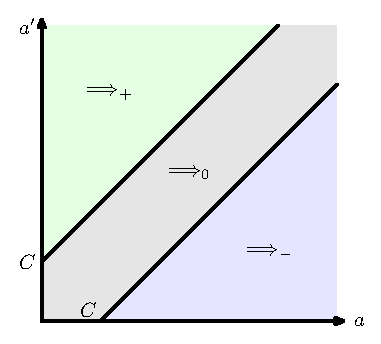
\includegraphics[scale=0.8]{figures-1.eps}
\caption{The three relations $\stepp +$, $\stepp -$, and $\stepp 0$.
The axes do \emph{not} correspond to the counters, 
but rather the initial and final values $a$ and $a'$ of a segment.}
\label{fig:areas}
\end{figure}


\para{Three types of segments}
Every segment $\rho_i \colon q(a) \reachrel q'(a')$, 
depending on the values of $a$, $a'$ and $a-a'$,
falls into one of three categories,
%split the relation $\step^\ast$ into three subrelations,
%which represent different kinds of \vass runs in $(Q\times\N^2)$:
denoted by $\stepp +$, $\stepp -$, and $\stepp 0$.
% We split the relation $\reachrel$ into three disjoint subrelations; 
% depending on the value of $a$, $a'$, and $a'-a$. 
If $q(a) \reachrel q'(a')$, we write:
\begin{equation}
\left.
\begin{aligned}\label{eq:tran0-+}
& q(a) \stepp 0\, q'(a'),\quad && \text{if\ \ $a\leq C$ or $a'\leq C$ or $|a'-a|\leq C $}\\
& q(a) \stepp - q'(a'),\quad && \text{if\ \ $a' > C$\ \ and\ \ $a > a'+C${}}\\
& q(a) \stepp + q'(a'),\quad && \text{if\ \ $a\phantom{'} > C$\ \ and\ \ $a' > a+C${}}
\end{aligned}\right\}
\end{equation}
See \Cref{fig:areas} for a graphical illustration.
% 
The precise definition of constant $C$ will be given in \Cref{sec:targetpump}.
Thus the rechability relation is 
\[
\reachrel^* \ = \ 
\big(\stepp 0 \ \cup \ \stepp - \ \cup \ \stepp + \big)^*,
\] 
an arbitrary composition
of the three sub-relations arbitrarily many times.
Note that the composition assures that \emph{control states match}.
% 
% \bigskip\noindent
Using this categorization 
we split the run $\rho$ into three \emph{phases} (possibly empty): 

\begin{itemize}
\item $\Phi_1$, which is the \emph{prefix} of $\rho$ and ends with the \emph{last} $\rho_i$ of the form $\stepp +$,
\item $\Phi_2$, which is an \emph{infix} of $\rho$ and consists only of $\rho_i$'s of the form $\stepp {0}^*$, 
\item $\Phi_3$, which is the remaining \emph{suffix} of $\rho$ starting 
with \emph{the first} $\rho_i$ of the form $\stepp -$.
% (followed by other \vass segments of the forms $\stepp -$ and $\stepp 0$).
\end{itemize}

\noindent
Clarly, the composition of the three phases yields
the reachability relation, that is
\begin{align} \label{eq:reachrel}
\reachrel^* \ = \ \Phi_1 \circ \Phi_2 \circ \Phi_3,
\end{align}
for  the three relations defined by the following rational expressions:
\begin{align*}
&\Phi_1 \ = \ ((\stepp 0 \ \cup \ \stepp -)^\ast \circ \stepp +)^\ast,\\
&\Phi_2 \ = \ (\stepp 0)^\ast,\\
&\Phi_3 \ = \ (\stepp - \circ \stepp {0}^\ast)^\ast.
\end{align*}

\para{Outline of decidability proof}

The proof uses semilinear sets.
Any subset of $\N^d$ of the form
\[
% \lin b {\{p_1,\dots,p_n\}} = 
\left\{ b + k_1 p_1 + \cdots + k_n p_n 
\mid k_1, \dots, k_n \in \N \right\},
\]
for $b, p_1, \dots, p_n \in \N^d$,
we call a
\emph{linear} set with base $b$ and periods $p_1, \dots, p_n$.
A \emph{semilinear} set is a finite union of linear sets in the same
dimension $d$.
We say $X \subseteq Q \times \N^d$ is semilinear 
if for every $q \in Q$, 
the set 
\(\{n \mid (q,n)\in X\} \subseteq \N^d\)
is semilinear.
Similarly, 
$R \subseteq (Q\times \N^d)^2$ is semilinear if for every $q,q' \in Q$,
the set
\( \{(n,n') \mid ((q,n),(q',n')) \in R \} \subseteq \N^{2d}\)
is semilinear.

\Cref{thm:main} is proved by showing that the relation $\Phi_2$, 
as well as
the image of relation $\Phi_1$ and pre-image of $\Phi_3$, are
\emph{effectively semilinear}, which means that they are 
semilinear sets and their descriptions are computable
given the underlying 2-\vass $\V$ and source and target
$s, t\in Q\times\N$.
Importantly, we only need to consider semilinar sets and relations
in dimension $d=1$.


\begin{lemma} \label{lem:0star}
$\Phi_2 \subseteq (Q \times \N)^2$ 
is an \emph{effectively semilinear} relation.
% The relation $\stepp {0}^*$ is effectively semilinear.
\end{lemma}


% \begin{lemma} \label{lem:compbackfor}
% One can compute 
% the set 
% $\big(\stepp - \ \circ \ \stepp {0}^*\big)^* \ \circ \ \{t\}$.
% \end{lemma}

\begin{lemma} \label{lem:compbackfor}
Given source $s$ and target $t$, the sets
\begin{alignat*}{6}
&\Phi_3 \circ \{t\} \ := \  \{y &&\mid (y,t) \in \Phi_3 \hskip 0.5pt\}  \ \subseteq \ Q \times \N, \\
&\{s\} \circ \Phi_1 \ := \  \{x &&\mid (s,x) \in \Phi_1 \} \ \subseteq \ Q \times \N
\end{alignat*}
are \emph{effectively semilinear}.
% One can compute 
% the set 
% $\{s\} \circ \big(\stepp {0}^* \ \circ \ E \ \circ \ \stepp +)^*$.
\end{lemma}

%  $\Phi_2 \subseteq (Q \times \N)^2$ 
% is an \emph{effectively semilinear} relation
% %\footnote{This means $\{n \in \N \colon (q,n) \in \Phi_3 \}$ is effectively semilinear, for every $q\in Q$.}%
% % 
% and that for given source $s$ and target $t$, the sets
% \begin{alignat*}{6}
% &\Phi_3 \circ \{t\} \ := \  \{y &&\mid (y,t) \in \Phi_3 \hskip 0.5pt\}  \ \subseteq \ Q \times \N, \\
% &\{s\} \circ \Phi_1 \ := \  \{x &&\mid (s,x) \in \Phi_1 \} \ \subseteq \ Q \times \N
% \end{alignat*}
% are also \emph{effectively semilinear}.

Relying on effective 
semilinearity given in \Cref{lem:0star,lem:compbackfor},
and on the effective equivalence of semilinear sets and Presburger 
Arithmetic \cite{},
the proof of \Cref{thm:main} is immediate:
the reachability question $s\reachrel^* t$
which, according to \eqref{eq:reachrel}, is equivalent to%
%\( (s,t) \in \Phi_1\circ\Phi_2\circ\Phi_3,\) \ie 
\begin{equation}
\exists\, x,y \in Q\times\N \ : \  x \in \{s\} \circ \Phi_1 \ \wedge \ (x,y) \in \Phi_2 
\ \wedge \ y\in \Phi_3 \circ \{t\},
\end{equation}
is effectively 
expressible in Presburger Arithmetic, and hence decidable \cite{}.
It thus remains to demonstrate the two key lemmas.


%Notationally, we allows ourselves to compose a relation $R\subseteq (Q\times\N)^2$ 
%with a set $X\subseteq Q\times\N$ to denote the set inverse image $R\circ X\subseteq Q\times\N$, 
%or the image $X\circ R \subseteq Q\times\N$.
%% Let $I_s = \{(s,s)\}$ be the relation containg exactly one pair, where $s$ is the source configuration.
%% Likewise, let $I_t = \{(t,t)\}$.
%We will be able to decide if $s\step^* t$, given source and target configurations $s,t\in Q\times\N$,
%as long as we prove the two following fact: one can (backward) compute the inverse image
%$E\circ \{t\}$, and (forward) compute the image 
%$\{s\} \circ \big(\stepp {0}^* \ \circ \ E \ \circ \ \stepp +)^*$,
%according to the partition into phases.




\section{Effective semilinearity} \label{sec:sl}

We denote by $\mysize \V$ the size of $\V$, in unary representation,
and by $\norm \V$ the max-norm of $\V$, namely the maximal absolute value of
all numbers appearing in transitions.
Clearly, $\mysize \V \geq \norm \V$.

We start with a basic observation concerning the building blocks
of sets of our interest:

\begin{lemma} \label{lem:0-+}
The relations $\stepp 0, \ \stepp -, \ \stepp +$ are effectively semilinear.
\end{lemma}
\begin{proof}
The relation $\reachrel$ is the reachability relation of a 2-\vass
$\V$, which is effectively semi-linear \cite{Blondin15}.
Each of the sub-relations $\stepp 0, \ \stepp -, \ \stepp +$ is a Presburger-definable subset of $\reachrel$,
and hence effectively semilinear as well.
\end{proof}


\para{Target and source pumping}


The \emph{target pumping} 
property of segments of the form $\stepp +$, is 
a central technical tool in the proofs of
\Cref{lem:0star,lem:compbackfor}:

\newcommand{\punkt}[2]{({#1}{\rightarrow}{#2})}
\begin{lemma} [Target pumping] \label{lem:targetpump}
Given a symmetric 2-\vass $\V$,
one can compute numbers $C, D \in \N$ 
such that for every pair of control states $q, q'$ of $\V$ and  
$a, a'\in\N$ such that $a > C$ and $a' > a + C$,%
\[
\punkt 1 2 \qquad
\text{if} \quad q(a,0)\step^* q'(0,a') \quad \text{then} \quad q(a,0) \step^* q'(0, a'+D),
\]
and similarly for the other three symmetric cases:
\begin{alignat*}{3}
&\punkt 2 2 \qquad
\text{if} \quad q(0,a)\step^* q'(0,a') \quad &&\text{then}  \quad  q(0,a) \step^* q'(0, a'+D),\\
&\punkt 2 1 \qquad
\text{if} \quad q(0,a)\step^* q'(a',0) \quad &&\text{then}  \quad  q(0,a) \step^* q'(a'+D, 0),\\
&\punkt 1 1 \qquad
\text{if} \quad q(a,0)\step^* q'(a',0) \quad &&\text{then}  \quad  q(a,0) \step^* q'(a'+D,0).
\end{alignat*}
Moreover, $C$ is polynomial in $\mysize \V$ and $D$ is exponential in $\mysize \V$.
\end{lemma}

In the sequel we fix the underlying symmetric 2-\vass $\V$ of
a symmetric 2-\cm.
The four claims of \Cref{lem:targetpump} jointly imply that 
$\stepp +$ is \emph{target-pumpable} in $\V$, 
that is for every pair of control states $q, q'$ of $\V$, 
% and  $a, a'\in\N$ such that $a, a'-a > C$, 
\begin{align} \label{eq:tpump}
q(a)\stepp + q'(a') \quad \implies  \quad  q(a) \stepp + q'(a'+D).
\end{align}
The reverse version of the four claims, where we swap source and target and reverse all transitions
(the reverse of $(q,w,q')$ is $(q',-w,q)$, as expected), 
implies that $\stepp -$ is \emph{source-pumpable}, that is 
\begin{align} \label{eq:spump}
q(a)\stepp - q'(a') \quad \implies  \quad  q(a+D) \stepp - q'(a').
\end{align}
Note that we can assume the same $D$ in \eqref{eq:tpump} and 
\eqref{eq:spump}, by taking the least common multiplicity of the
two constants given by the two applications of \Cref{lem:targetpump}.
In the sequel, fix the constant 
$D$ from \eqref{eq:tpump} and \eqref{eq:spump}.


\para{Periodic sets}

A set $X \subseteq Q \times \N$ is $N$-periodic if
for all $(q,a) \in X$, also $(q,a+N) \in X$.
It is a folklore that semilinear sets $X\subseteq Q\times\N$
are $N$-periodic for some period $N$. 
In the sequel it will be crucial that all semilinear sets we maintain
are $D$-periodic with the same period $D$.
% 
For instance, in consequence of \eqref{eq:tpump} and \eqref{eq:spump}, 
the image $S\circ \stepp +$ as well as the pre-image
$\stepp - \circ S$ is always $D$-periodic, irrespectively of
$S\subseteq Q\times\N$.
% 
%Now define the three phases $\Phi_1, \Phi_2, \Phi_3$ as stated above.
%
%\begin{align} \label{eq:3phases}
%\big(\stepp {0}^* \ \circ \ E \ \circ \ \stepp +)^* \ \circ \ \stepp {0}^* \ \circ \ E
%\end{align}
%where 
%\[
% E  \ = \ \big(\stepp - \ \circ \ \stepp {0}^*\big)^*.
%\]
%Thus we split every run into three phases: the first one ends with the last appearance of $\stepp +$,
%the middle one consisting just of $\stepp {0}^*$, and the last one starting with $\stepp -$ and
%iterating arbitratily many times $\stepp -$ and $\stepp 0$.
%Each of the phases may be empty.
% 

A $D$-periodic set $X$ is representable by a function 
$\minf X : Q\times \setfromto 0 {D-1} \to \N \cup \{\infty\}$ 
that maps a state $q\in Q$ and $r<D$ to the least number $n$ 
whose reminder modulo $D$ equals $r$, and such that $(q,n)\in X$ 
(and to $\infty$ if there is no such number):
\[
\minf X (q,r) \ = \ \min\{n : (q,n) \in X, \ \ n \equiv r\!\!\mod D\}.
\]
In the proofs of \Cref{lem:0star,lem:compbackfor}
we compute increasing (actually, non-decreasing) chains 
of $D$-periodic sets of configurations $X\subseteq Q\times\N$.
%We represent these sets in vector form as functions
%$X:Q\to \powset{\N}$, where $X(q)$ is pumpable for every $q\in Q$, namely $a\in X(q)\implies a+D\in X(q)$.
Termination of computation is guaranteed by:
%  the following lemma:
\begin{lemma} \label{lem:stab}
    Every non-decreasing chain of $X_1 \subseteq X_2 \subseteq \cdots$ of $D$-periodic sets of $\N$ stabilizes.
\end{lemma}
% 
\begin{proof}
The sequence $\minf {X_1}, \minf{X_2}, \ldots$ is a non-increasing
chain of functions, ordered pointwise 
(assuming $n<\infty$ for $n\in\N$), 
and hence necessarily stabilises due to well-foundedness
of the function space $Q\times \setfromto 0 {D-1} \to \N \cup \{\infty\}$.
\end{proof}


\begin{proof}[Proof of \Cref{lem:0star}]
    \vrm{Hard; to write down later.}\par
    Computable by a 1-counter automaton, a special case of a pushdown automaton.
\end{proof}

\begin{proof}[Proof of \Cref{lem:compbackfor}]
Recall that $\big(\stepp - \ \circ \ \stepp {0}^*\big) \ \circ \ S$
is the set of all 
\((q,a) \in Q \times \N\) such that $q(a)$ leads to some $x \in S$ via a run of form $(\stepp -\stepp {0}^\ast)^\ast$.
Thus, $\big(\stepp - \ \circ \ \stepp {0}^*\big) \ \circ \ S$ is source-pumpable 
due to \eqref{eq:spump},
irrespectively of $S$.

It is also computable due to \Cref{lem:0-+,lem:0star}, 
as long $S$ is semilinear.
This is seen by iterating the computation of the transformation
\[
S \quad \mapsto \quad \big(\stepp - \ \circ \ \stepp {0}^*\big) \ \circ \ S
\quad \cup \quad S,
\]
which stabilises, by \Cref{lem:stab}.
\vrm{how many details to write here? $\stepp {0}^\ast$ has a representation as a semilinear set;
to explain why every intermediate step in fixed point computation also has an efficient representation,
and give it.}
Furthermore, by the effective representation of $\stepp {0}^\ast$ and $\stepp {-}$ as semilinear relations,
each step of the process above is effectively representable,
and thus so is the fixed point.
\end{proof}

\begin{proof}[Proof of \Cref{lem:compbackfor}]
Again, The set $f(S) = S \ \circ \ \stepp {0}^* \ \circ \ E \ \circ \ \stepp +$ is
target-pumpable due to \eqref{eq:tpump},
irrespectively of $S$.
Computability is more involved, but relates again on iteration of the transformation
\[
S \quad \mapsto \quad f(S) \quad \cup \quad S,
\]
relying on \Cref{lem:stab}.

\vrm{To write that $f(S)$ consists of arithmetic progressions of period $D$,
and that we choose the minimal element of every arithmetic progression.}
To compute $f(S)$, one first establishes which remainders modulo $D$ appear in this set,
by applyting the transformation of \Cref{lem:compback} to the set 
$(\stepp + \ \circ \ M_k)$,
where $M_k$ contains all numbers equal to $k$ modulo $D$, and checking intersection with 
the set $(S\ \circ \ \stepp 0)$. 
Then, by exhaustive search one finds the smallest number in $f(S)$, 
for each remainder modulo $D$ separately.
\end{proof}


        
%\noindent A \emph{Counter Machine with $n$-counters} (or $n$-\cm for short) 
%is a quadruple
%\[
%\mathcal{M} = (Q, q_0, q_h, \Delta)
%\]
%where:
%\begin{itemize}
%    \item $Q$ is a finite set of \emph{control states},
%    \item $q_0 \in Q$  and $q_h \in Q$ are the \emph{initial} and the \emph{halting} state respectively,
%    \item $\Delta \subseteq (Q - \{q_h\}) \times \text{Instr}_n \times Q$ is the 
%    \emph{transition relation}, where $\text{Instr}_n$ is a finite subset of 
%    $\Z^n \cup \{ \text{\lq\lq$\textsf{c}_i=0$?\rq\rq} \mid 1 \leq i \leq n\}$.
%\end{itemize}
%
%A configuration of $\mathcal{M}$ is a pair $(q,x)$ where $q \in Q$ and $x \in \N^n$.
%A run of $\mathcal{M}$ is a sequence $\rho=c_0, c_1, \dots, c_\ell$ of configurations,
%where $c_0=(q_0, (0,0))$,
%and if $c_i = (q_i,x_i)$, then $c_{i+1}=(q_{i+1},x_{i+1})$
%for some transition $(q_i, A,q_{i+1}) \in \Delta$,
%where:
%\begin{itemize}
%\item $x_{i+1} = x_i + A$, if $A \in \Z^n$,
%\item $x_{i+1}= x_i$ and $x_i(j)=0$ if $A = \text{``$\textsf{c}_j=0?$\rq\rq}$.
%\end{itemize}
%We say $\rho$ is an accepting run if $q_\ell = q_h$.
%
%An $n$-\vass is an $n$-\cm with $\Delta \subseteq Q \times \Z^n \times Q$.
%



%\para{1-dimensional notation}
%By symmetry, \Cref{lem:targetpump} holds more generally:
%for every pair of control states $q$, $q'$ of $\V$ and  
%$a, a'\in\N$ such that $a$, $a'-a>C$, 
%\begin{align*}
%q(0,a)\step^* q'(0,a') \quad \implies  \quad  q(0,a) \step^* q'(0, a'+D)\\
%q(0,a)\step^* q'(a',0) \quad \implies  \quad  q(0,a) \step^* q'(a'+D, 0)\\
%q(a,0)\step^* q'(a',0) \quad \implies  \quad  q(a,0) \step^* q'(a'+D,0).
%\end{align*}
%As discussed before, the ``zero-testing states'' indicate which counter is zero, 
%so we can merge the four cases into one notation, 
%adopting the shorthand \eqref{eq:basictran}.
%and that a run zero tests every counter whenever it has value 0. 
% To this aim double the control states, that is replace every $q\in Q$
% by $q_1, q_2$, each of them involved into the same increment transitions as $q$, but $q_1$ only 
% capable to do those zero-testing transitions $q$ that test counter 1, and likewise $q_2$ only 
% capable to do those zero-testing transitions $q$ that test counter 2.

%So prepared, we can simply write
%\begin{align} \label{eq:basictran}
%q(a) \step^* q'(a')
%\end{align}
%without specifying which of the four cases is happening
%\begin{align*}
%q(a,0)\step^* q'(0,a')\\
%q(0,a)\step^* q'(0,a')\\
%q(0,a)\step^* q'(a',0)\\
%q(a,0)\step^* q'(a',0)
%\end{align*}
%since the control states $q,q'$ uniquely determine these two bits of information.
%Note that the newly introduced zero tests are not symmetric, but we do not assume that. 

% \begin{figure}
% \centering
% 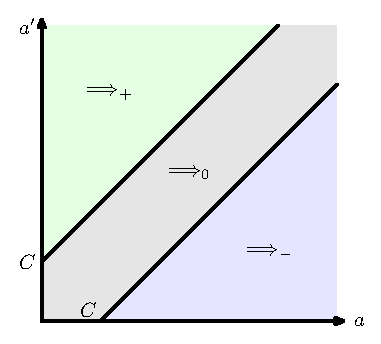
\includegraphics{figures-1.eps}
% \caption{The three relations $\stepp +$, $\stepp -$, and $\stepp 0$.
% The axes do \emph{not} correspond to the counters, 
% but rather the initial and final values $a$ and $a'$ of the \vass segment.}
% \label{fig:areas}
% \end{figure}

%Each of the three relations \eqref{eq:tran0-+} is included in $(Q\times\N)^2$.

% \para{VASS}
% In a \vass $\V$, \emph{path} is a sequence of transitions 
% where the target state of every transition
% matches the source targe state of the next one.
% A \emph{run} is a path plus a source configuration whose
% state matches with the first transition, such that
% all transitions are fireable.
% A \emph{cycle} is a path where the source state of the 
% first matches the target state of the last one.
% By $c; c'$ we denote the concatenation of paths $c, c'$, and  
% by $c^k$ we denote the $k$-fold concatenation of a cycle $c$.
% Firing of a single transition $q \xstep{(x_1,x_2)} q'$
% we call a \emph{step} and
% write $q(n_1, n_2) \step q'(n_1+x_1, n_2+x_2)$;
% and $\step^\ast$ is the transitive closure of $\step$.

% \medskip


% \para{Relations}
% If $R\subseteq X \times Y$, $R' \subseteq Y \times Z$ and $A \subseteq X$, $B \subseteq Y$,
% we define the following compositions:
% \begin{alignat*}{3}
% & R \circ R' &&= \{(x,z) \mid \exists y : (x,y) \in R \wedge (y,z) \in R'\},\\
% & R \circ B  &&= \{x \in A \mid \exists y \in B : (x,y)\in R\},\\
% & A \circ R  &&= \{y \in B \mid \exists x \in A : (x,y)\in R \}.
% \end{alignat*}
% If $X=Y$, then $R^\ast$ is $\bigcup_{n=0}^\infty \underset{\text{$n$ times}}{\underbrace{R \circ \cdots \circ R}}$.





\section{Target pumping: Proof of \Cref{lem:targetpump}}\label{sec:targetpump}
%

% We now prove \Cref{lem:targetpump}.
We focus on proving point $\punkt 2 2$, noticing however that
literally the same argument 
works for point $\punkt 1 2$.
\sla{swapped $\punkt 1 2$ with $\punkt 2 2$}
The other two points, namely $\punkt 2 1$ and $\punkt 1 1$,
follow immediately by swapping the coordinates.
% \mei{I don't think the symmetry assumption is necessary
% for this particular step.}
% \sla{right, i've removed the symmetry assumption.}

To ease the presentation, we introduce the following definitions:
\begin{itemize}
\item For a transition $t = (q, \updinstr{w}, q') \in T$, the states $q, q'$
    are said to be the \emph{source} and \emph{target} of $t$ respectively,
    and the vector $w$ is said to be the \emph{effect} of $t$.
\item A \emph{path} is a sequence of transitions such that the target
    of each transition matches the source of the next transition
    in the sequence. Unlike a run, a path does not fully specify
    the source and target configurations.

    The source of the first transition is said to be the \emph{source of the path},
    and the target of the final transition is said to be the \emph{target of the
    path}. The \emph{effect of a path} is defined as the sum of the effects of its
    transitions.
\item A \emph{cycle} is a path whose source and target coincide.
\item A path $\rho$ is said to be \emph{fireable} at a configuration $q(\vr v)$
    if there exists a configuration $q'(\vr v')$ such that $q(\vr v) \xstep{\rho} q'(\vr v')$,
    \ie $\rho$ can be executed starting from $q(\vr v)$, without the counters
    having to go negative along the way.
    We denote the target configuration $q'(\vr v')$ thus obtained by $q(\vr v); \rho$.
\item For paths $\rho_1$ and $\rho_2$, denote their concatenation by $\rho_1; \rho_2$.
% \item A path $\rho_2$ is said to be \emph{fireable after} a path $\rho_1$, if for any
%     configuration $q(\vr v)$ at which $\rho_1$ is fireable, the concatenation
%     $\rho_1; \rho_2$ is fireable as well.
\item For a path $\rho$, the \emph{transposed path} $\overline{\rho}$ is obtained
    by applying the symmetry assumption at each transition.
    If $\rho$ has effect $(a, b)$, $\overline{\rho}$ has effect $(b, a)$.
\end{itemize}

We define the \emph{norm} of a vector $w = (w_1,w_2) \in \Z^2$ 
to be the maximal absolute value of its components,
$\norm{w}=\max\{|w_1|,|w_2|\}$, and 
the norm of a 2-\vass $\V=(Q,T)$ to be the maximal norm of the effects 
of its transitions, 
$\norm \V = \max\{\norm{w} \mid (q,\updinstr{w},q')\in T\}$.


\begin{proof}[Proof of \Cref{lem:targetpump} $\punkt 2 2$]
Consider a fixed symmetric 2-\vass $\V = (Q,T)$ and
a run $\sigma : q(0,a)\step^* q'(0,a')$ for some $a, a'\in \N$.
Assuming that the difference $a'-a$ is sufficiently large
(namely larger than some $C$, depending only on $\V$),
we modify the run to lift the target configuration to $q'(0,a'+\gamma D_\sigma)$ for any
multiple $\gamma \in \N$ of some particular $D_\sigma$, which depends on both $\V$ and $\sigma$.
Holding $\V$ fixed, $D_\sigma$ will only attain finitely many different values,
hence we argue that taking the least common multiple of all $D_\sigma$ yields a
constant $D$ satisfying the claim of the lemma.

Denote by $\widetilde \sigma$ the sequence of transitions fired along
the run $\sigma$, obtaining its corresponding path.
According to the linear-path-scheme (LPS) decomposition of 
\cite[Thm.~1]{Blondin15}, 
we may assume \mywlog that 
$\widetilde\sigma$ is built of paths 
$t_0, \ldots, t_\ell$ and cycles $c_1, \ldots, c_\ell$:
\begin{align}\label{eq:lps}
\widetilde\sigma \ \in \ t_0 \ c_1^* \ t_1 \ c_2^* \ \ldots \ c_\ell^* \ t_\ell,
\end{align}
where the lengths of each path $t_i$ and cycle $c_j$ are at most $e$,
and both $\ell$ and $e$ are bounded by a polynomial of $\mysize \V$,
the size of the unary representation of $\V$.
Note that we do not claim any bound the number $n_j$ of iterations
in $\widetilde\sigma$ of the cycles $c_j$.

Let $C_0 \leq e \norm \V$ be the minimal value such that every cycle of $\V$
of length at most $e$ is \emph{fireable} at $\vr v_0=(C_0, C_0)$.
Call a cycle $c_j$ \emph{major} if its number of iterations $n_j$ is larger
than $2 C_0$, and \emph{minor} otherwise.
\Mywlog we may assume that all cycles are major,
by inlining any minor cycles $c_i$ into their neighboring one-off paths $t_{i-1}$ and $t_i$.
After this operation, lengths of the one-off paths are bounded by
$e' := 2e (C_0 + 1)$.

Call a cycle $c_j$ \emph{sum-increasing} if its effect $(x_j, y_j)$ satisfies $x_j + y_j > 0$.
We claim that, by setting a large enough value of $C$, we can guarantee that the run
will contain at least one (major) sum-increasing cycle.

Indeed, we are assuming that $a' - a > C$, the sum of counters
must increase by more than $C$ along $\sigma$.
% In particular, the total effect of the one-off paths
% $t_0, \ldots, t_\ell$ is bounded,
% as each of them may increase the sum of the counters by at most $2 e \norm \V$.
% Likewise, a single iteration of a cycle may only increase the sum of the counters by at most
% $2 e \norm \V$, and each minor cycle gets executed at most $2 C_0$ times.
Thus, it is enough when
\[
    C \ \geq \ C_1 \ := \ 
    e'_\mathrm{max} 2\norm\V (\ell_\mathrm{max} + 1),
\]
where $e'_\mathrm{max}$ and $\ell_\mathrm{max}$ are the (polynomial in $\mysize\V$) bounds
on $e'$ and $\ell$, respectively.
\lukasz{Does it make sense to introduce $e'_\mathrm{max}$ and $\ell_\mathrm{max}$?
It is enough to say that $\ell$ and $e'$ are polynomially bounded 
to avoid introducing new variables.
}


We now focus our attention on the sum-increasing cycles, and perform
case analysis in terms of the sign of each coordinate of their effect.
Specifically, the effect of a \emph{sum-increasing} cycle can be:
vertical $(0,+)$, horizontal $(+,0)$, or one of $(+,-)$, $(+,+)$, or $(-,+)$.
We classify these into three cases.

\para{Case 1: Some sum-increasing cycle $c_j$ has vertical $(0,+)$ effect}
One extra iteration of this cycle yields the claim, with the vertical effect
of the cycle determining $D_\sigma$.

\para{Case 2: Some sum-increasing cycle $c_j$ has effect $(-,+)$ or $(+,-)$}
Assume that $c_j$ has effect $(-x,y)$ for some positive integers $x,y$.
Observe that $y > x$.
The case of $(+,-)$ effect is analogous.
% 
For our argument it is enough if the $n_j$ is large enough to guarantee that 
somewhere in the middle of $c_j^{n_j}$, the 
transposed cycle $\overline{c_j}$ becomes fireable.
We observe the following key claim, relying on the fact that  
the effect of $c_j$ is nonzero on both coordinates
(in particular note that we do not use the sum-increasing
assumption for this claim):
%
\begin{claim}  \label{claim:fireable}
    If $c_j^{n_j}$ is fireable at $q(\vr v)$, then for any
    repetition count $i$ satisfying
    $C_0 \leq i \leq n_j - C_0$,
    the transposed cycle $\overline{c_j}$ is fireable at $q(\vr v); c_j^i$.
\end{claim}
%
\begin{proof}
The $n_j+1$ configurations at the boundaries between
the iterations of $c_j$ within $c_j^{n_j}$
form an arithmetic progression given by
$(x_i, y_i) = (x_0 - i x, y_0 + i y)$.
%For a coordinate at which the
%effect of the cycle is positive, say $x > 0$, we obtain $x_i \geq C_0$
%for $i \geq C_0$. On the other hand, for a coordinate with a negative effect,
%say $y < 0$, we have $y_i = y_{n_j} - (n_j - i)y$, with $y_{n_j} \geq 0$, and
%thus $y_i \geq n_j - i$. Hence for $i \leq n_j - C_0$ we have $y_i \geq C_0$.
%As such, for $C_0 \leq i \leq n_j - C_0$, both coordinates are above $(C_0, C_0)$,
%which suffices to obtain that $\overline{c_j}$ is fireable.
%It suffices to show that for appropriate $i$ we have $x_i, y_i \geq C_0$.
%For coordinates at which the effect of $c_j$ is positive, say $x > 0$,
%It suffices that $C_0 \leq i \leq n_j - C_0$, as then we have
%$x_i = x_0 - i x \leq x_0 - i \geq C_0$ and 
Observe that for $C_0 \leq i \leq n_j - C_0$
we have $y_i = y_0 + iy \geq y_0 + i \geq C_0$ 
and $x_i = x_0 - ix \geq x_0 + (C_0 - n_j)x \geq C_0$.
%
%Similarly, for coordinates with negative effect, say $y < 0$,
%it's enough that $i \leq n_j - C_0$.
\end{proof}

Recall now that, having eliminated all minor cycles by inlining,
we have $n_j > 2C_0$ and therefore
the range of values of $i$ admissible for \Cref{claim:fireable}
is non-empty. Setting $i := C_0$, we have that the transposed cycle
$\overline{c_j}$ is fireable after the first $C_0$ iterations
of $c_j$ within $\sigma$. Equivalently, the concatenation $c_j; \overline{c_j}$
is fireable after $c_j^{C_0}$.

Recall we have that $y > x$, as the cycle is
sum-increasing. Thus, the effect of $c_j; \overline{c_j}$, being $(y-x, y-x)$,
is positive on both coordinates, and $c_j; \overline{c_j}$ may be fired arbitrarily
many times in the middle of $c_j^{n_j}$, without interference with the remainder of $\sigma$.
% Explicitly "in the middle", not "at the midpoint", the latter might not even exist
% if n_j happens to be odd.

% Let $k$ be the least common multiplicity of $m_2 - m_1$ and $m_1$.  
Now set $u:=x(y-x)$.
By iterating $x$ times the cycle $c_j; \overline{c_j}$,
we get a cycle with effect $(u,u)$, and then appending
$c_j^{y-x}$ we get the desired vertical effect.
Indeed, the effect of
\[
\big(c_j; \overline{c_j}\big)^{x}; c_j^{y-x}
\]
is $(0, (x+y)(y-x))$, and this cycle is still fireable in the middle of
$c_j^{n_j}$.
We thus get the claim with $D_\sigma = (x+y)(y-x)$.

\begin{figure}[h]
\centering
\begin{tikzpicture}[
    >=stealth,
    scale=0.8,
    every node/.style={font=\small}
]
    \begin{scope}
        \fill[green!10] (0,0) rectangle (3,2);
        \fill[green!10] (0,0) rectangle (-3,-2);
        \fill[red!10] (0,0) rectangle (-3,2);
        \fill[red!10] (0,0) rectangle (3,-2);
      % axes
      \draw[->] (-3,0) -- (3,0) node[right] {$x$};
      \draw[->] (0,-2.0) -- (0,2.0) node[above] {$y$};

      % rays corresponding to steepnesses
      \draw[dashed] (0,0) -- (1.75,2.0)
          node[pos=.92, right] {$\varphi_1$};

      \draw[dashed] (-1.2,-0.6) -- (2.4,1.2)
          node[pos=1.0, below] {$\varphi_2$};

      \draw[dashed] (0,0) -- (2.5,-1.3)
          node[pos=1.0, below] {$\varphi_3$};

      % cycle effects
      \draw[->, very thick] (0,0) -- (-1.3,-1.5)
          node[pos=.82, right] {$c_1$};

      \draw[->, very thick] (0,0) -- (1.8,0.9)
          node[pos=.82, below] {$c_2$};

      \draw[->, very thick] (0,0) -- (-1.8,0.95)
          node[pos=.62, above] {$c_3$};

      % angle / steepness indication
      % \node at (6.1,2.3) {$\varphi_1>\varphi_2>\varphi_3$};

      % labels
      % \node[below right] at (4.3,0.34) {horizontal effect};
      % \node[above left] at (-0.2,2.09) {vertical effect};

        % sign labels
        \node[scale=0.8] at (2.1,-0.3) {$x_2>0$};
        \node[scale=0.8] at (-2.0,-0.3) {$x_1,x_3<0$};
    \end{scope}

    \begin{scope}[xshift=8cm]
        \draw[->] (-2.5,0) -- (2.5,0) node[right] {$x$};
        \draw[->] (0,-2) -- (0,2) node[above] {$y$};

        \coordinate (a) at (2.0,1.0);
        \draw[->, thick, dotted, green!50!black] (a) -- (0, 1.5)
            node[left] {$\checkmark c_{j_1}$};
        \draw[->, thick, dotted, green!50!black] (a) -- (0, 0.7)
            node[left] {$\checkmark c_{j_2}$};
        \draw[->, thick, dotted, red!50!black] (a) -- (0, -1.0)
            node[left] {$\times c_{j_3}$};
        \draw[->, very thick] (0,0) -- (a)
            node[right] {$c_i$};
    \end{scope}
\end{tikzpicture}
\caption{
  The steepness comparison central to the proof strategy of Case 3.
  Left: An illustration of the properties of steepness.
  The vectors represent the effects of three cycles
  $c_1$, $c_2$, and $c_3$, where $c_2$ is horizontally
  positive, and the other two are horizontally negative.
  The cycle $c_1$ is steeper than $c_2$, and $c_2$ is steeper than $c_3$.
  Cycles whose effect lies within the area shaded green (resp. red) have positive (resp. negative) steepness.
  Right: A horizontally-positive sum-increasing cycle $c_i$,
  with three candidates for a subsequent horizontally-negative cycle $c_j$, illustrated
  in terms of their combined effect
  (when combined with coefficients chosen to put said effect on the vertical axis).
  Observe how the vertical effect obtained this way is positive exactly
  when $c_i$ is steeper than $c_j$ (cf. \Cref{claim:steep}).
}
\label{fig:steep}
\end{figure}

\para{Case 3: All sum-increasing cycles have $(+,0)$ or $(+,+)$ effect}
Let us restrict our attention to those cycles $c_j$, whose effect 
$(x_j,y_j)$ satisfies $x_j\neq 0$.
Depending on whether $x_j>0$ or $x_j<0$, we call such cycles 
\emph{horizontally positive}, or \emph{horizontally negative} respectively.
Define the \emph{steepness} of such cycles $c_j$ as $y_j/x_j$, and denote it by $\varphi_j$.
Note that, while in general the steepness may be negative,
by assumption it will never be negative for a sum-increasing cycle
(see \Cref{fig:steep}, left).

We will now aim at increasing 
the repetition count of one of the sum-increasing
cycles, together with one other cycle, occurring later in the run, 
in order to obtain a vertical effect (see \Cref{fig:steep}, right).
That suitable cycles exist is stated by the following claim.

\begin{figure}[t]
\centering
\begin{tikzpicture}[
    >=stealth,
    scale=0.9,
    every node/.style={font=\small}
]

% ------------------------------------------------------------
% Run in configuration space
% ------------------------------------------------------------

% Axes
\draw[->] (0,0) -- (11.8,0) node[right] {$x$};
\draw[->] (0,0) -- (0,4.5) node[above] {$y$};

% Configurations along the run
\coordinate (P0) at (0.0,2.1);
\coordinate (P1) at (0.5,1.0);
\coordinate (P1e) at (4.2,1.4);
\coordinate (P2) at (4.7,2.2);
\coordinate (P2e) at (7.0,4.5);
\coordinate (P3) at (8.0,5.0);
\coordinate (P3e) at (7.2,2.0);
\coordinate (P4) at (8.2,2.2);

% Ordinary path segments
\draw[dotted,->] (P0) -- (P1);
\draw[->,very thick] (P1) -- (P1e) node[pos=.55,below] {$c_1^{n_1}$};
\draw[dotted,->] (P1e) -- (P2);
\draw[->,very thick] (P2) -- (P2e) node[pos=.45,right] {$c_2^{n_2}$};
\draw[dotted,->] (P2e) -- (P3);
\draw[->,very thick] (P3) -- (P3e) node[pos=.55,right] {$c_3^{n_3}$};
\draw[dotted,->] (P3e) -- (P4);


% ------------------------------------------------------------
% Configuration labels
% ------------------------------------------------------------

\fill (P0) circle (1.5pt);
\fill (P1) circle (1.5pt);
\fill (P2) circle (1.5pt);
\fill (P3) circle (1.5pt);
\fill (P1e) circle (1.5pt);
\fill (P2e) circle (1.5pt);
\fill (P3e) circle (1.5pt);
\fill (P4) circle (1.5pt);

\node[above right] at (P0) {$(X_0, Y_0)=(0, a)$};
\node[below right]      at (P1e) {$(X_1, Y_1)$};
\node[above left]      at (P2e) {$(X_2, Y_2)$};
\node[below] at (P3e) {$(X_3, Y_3)$};

  % angle / steepness indication
  \node at (11,5.0) {$\varphi_1<\varphi_2<\varphi_3$};

\end{tikzpicture}

\caption{A hypothetical run violating \Cref{claim:steep}.
Thick lines represent iterated cycles, and dotted lines represent 
one-off paths.
The cycles $c_1$ and $c_2$ are 
horizontally positive and sum-increasing, the latter steeper than
the former, and $c_3$ is a horizontally negative (sum-decreasing) cycle
steeper than both $c_1$ and $c_2$.
% Thus none of sum-increasing cycles is followed by a less steep
% horizontally negative cycle.
Observe how this run gets further away from the Y axis as it progresses.
Intuitively, runs violating \Cref{claim:steep} like this one are ruled out, because
we're considering runs that end \emph{on} the Y axis,
above the starting point of the run.
To extend the run and have it reach such an endpoint, one would need to extend it
with a horizontally-negative cycle that's either 
less steep than $c_2$, or sum-increasing, with the latter option
putting the run in the purview of Case 2.}
\label{fig:steep-counterexample}
\end{figure}


\begin{claim} \label{claim:steep}
    There are some $i<j$ such that $c_i$ is a sum-increasing cycle, $c_j$ is
    horizontally negative, and $c_i$ is steeper than $c_j$ (\ie $\varphi_i > \varphi_j$).
\end{claim}
%
\begin{proof}
%Then, for any horizontally negative cycle $c_j$,
Call a sum-increasing cycle \emph{record-breaking} if it is
steeper than all sum-increasing cycles that came before it,
and suppose that the claim doesn't hold
(see \Cref{fig:steep-counterexample} for illustration).
In outline, we will define a sequence of straight lines in the configuration space,
each parallel to the effect of the most recent record-breaking cycle,
such that the counter values will always stay below the current line.
We will then show that the supposed target configuration of the run
is above the final line, to derive a contradiction.
\mei{TODO Figure. Probably add to \Cref{fig:steep-counterexample}?}

To this end, for a cycle $c_i$, denote by $\beta_i$ the steepness of
the most recent record-breaking cycle, \ie
\[
    \beta_i = \begin{cases}
        \max(\beta_{i-1}, \varphi_i) & \text{if $c_i$ sum-increasing} \\
        \beta_{i-1} & \text{otherwise}
    \end{cases}
\]
with $\beta_0 = 0$ as the initial value.
As one would expect, the value of $\beta_i$ will define the slope of each line.
Concretely specifying the $y$-intercept, however, requires a bit more work.

Define $(X^\pre_i, Y^\pre_i)$ and $(X^\post_i, Y^\post_i)$ to be the counter values
the run achieves immediately before and after $c_i^{n_i}$, respectively.
Let $k$ be the index of the first sum-increasing cycle of the run.
For $i \geq k$, define $S_i \leq C_1$ as the sum of the norms of
the effects of all one-off paths between $c_k$ and $c_i$, \ie,
writing $\norm {t}$ for the sum of norms of transitions along a path $t$,
\[
    S_i = \sum_{j=k}^{i-1} \norm{t_j}
\]
We extend the definitions in a natural way to $i = \ell + 1$ where relevant:
let $(X^\pre_{\ell + 1}, Y^\pre_{\ell + 1})$ be the counter values
of the run's target configuration, and denote by $S_{\ell + 1}$
the sum of norms of effects of all one-off paths after $c_k$, up to and
including $t_\ell$.

% Note that, if \Cref{claim:steep} indeed doesn't hold, we have $\beta_j \leq \varphi_j$ for any
% horizontally negative cycle $c_j$.
% Indeed, for $c_j$ occurring after $c_{k_1}$, we would otherwise get
% $\varphi_i = \beta_j > \varphi_j$, which satisfies \Cref{claim:steep}.
% On the other hand, for $c_j$ before the first sum-increasing cycle,
% we only need to show $-1 \leq \varphi_j$. But horizontally negative
% cycles of steepness lower than $-1$ are sum-increasing, and for
% the current case we are assuming that all sum-increasing cycles
% are horizontally positive.
%
% On the other hand, for a horizontally \emph{positive} cycle $c_j$,
% we have $\varphi_j \leq \beta_j$, either by definition, for sum-increasing cycles,
% or trivially, as $\varphi_j \leq -1 \leq \beta_j$ for 
% horizontally positive cycles $c_j$ that are not sum-increasing.

By induction on $i \geq k$, we will now prove that the pair $(X^\pre_i,Y^\pre_i)$ of
counter values will always satisfy
\begin{equation} \label{eq:steep-ind}
    Y^\pre_i \, \leq \, Y^\pre_k \, + \, S_i (1 + \beta_i) \, + \, \beta_i X^\pre_i.
\end{equation}

At $i = k$, the inequality trivially holds.
Suppose then that the inequality holds at a specific $i \geq k$,
aiming to prove it for $i+1$.

We shall follow the structure of the run, aiming first to prove
that $(X^\post_i, Y^\post_i)$ stays below the same line, \ie
\begin{equation} \label{eq:steep-ind-post}
    Y^\post_i \, \leq \, Y^\pre_k \, + \, S_i (1 + \beta_i) \, + \, \beta_i X^\post_i.
\end{equation}
\mei{This step would work well as a figure, I'll try to find the time to make one.}
Writing $X^\post_i = X^\pre_i + n_i x_i$ and $Y^\post_i = Y^\pre_i + n_i y_i$, we see that
our aim is to prove $y_i \leq \beta_i x_i$.
The first case, easily handled, is when $x_i = 0$. Indeed, we handle cycles of vertical effect
$(0, +)$ in Case 1, so if we encounter such a cycle here, then $y_i \leq 0$ must hold.

In the interesting case where $x_i \neq 0$, we apply the definition
of $\varphi_i$ to express the desired inequality as $\varphi_i x_i \leq \beta_i x_i$,
and consider the sign of $x_i$.
For a horizontally positive cycle, \ie $x_i > 0$, we need $\varphi_i \leq \beta_i$.
If $c_i$ is sum-increasing, this holds by definition;
otherwise note $\varphi_i \leq 0 \leq \beta_i$.

Finally, let $c_i$ be a horizontally negative cycle. In that situation, we need
$\varphi_i \geq \beta_i$.
Let $j$ be the most recent record-breaking cycle before $i$, which must
exist, as $i \geq k$ (and $i = k$ is ruled out by $c_i$ being horizontally negative).
Now note that if we had $\varphi_i < \beta_i = \varphi_j$, cycles $c_j$ and $c_i$
would satisfy \Cref{claim:steep}. As we are assuming that the claim doesn't hold,
we indeed have $\varphi_i \geq \beta_i$, thereby establishing \eqref{eq:steep-ind-post}.
\mei{$i$ and $j$ ended up having the opposite meaning to the statement of the claim,
maybe we should swap them.}
\sla{no need to swap}

Our next focus shall be proving that
\begin{equation} \label{eq:steep-ind-pre1}
    Y^\pre_{i+1} \, \leq \, Y^\pre_k \, + \, S_{i+1} (1 + \beta_i) \, + \, \beta_i X^\pre_{i+1}.
\end{equation}
With $(\Delta x, \Delta y)$ denoting the effect of the one-off path $t_i$,
we have $X^\pre_{i+1} = X^\post_i + \Delta x$, and analogously,
$Y^\pre_{i+1} = Y^\post_i + \Delta y$. Comparing with \eqref{eq:steep-ind-post}, we
see that it'll suffice to show
\[
    \Delta y \, \leq \, \norm{t_i} (1 + \beta_i) \, + \, \beta_i \Delta x
\]
(recall that $S_{i+1} = S_i + \norm{t_i}$). As both $|\Delta x|$ and $|\Delta y|$
are bounded by $\norm{t_i}$, we have
\begin{align*}
    \Delta y \, &\leq \, \norm{t_i}, \\
    - \Delta x \, &\leq \, \norm{t_i}.
\end{align*}
Multiplying the latter by $\beta_i$ and adding the two inequalities together,
we obtain
\[
    \Delta y - \beta_i \Delta x \, \leq \norm{t_i} (1 + \beta_i),
\]
as required.

Having now established \eqref{eq:steep-ind-pre1}, we note that
$\beta_i \leq \beta_{i+1}$, and moreover both
$S_{i+1}$ and $X^\pre_{i+1}$ are nonnegative, so we have
\[
    \begin{split}
        Y^\pre_{i+1} \, &\leq \, Y^\pre_k \, + \, S_{i+1} (1 + \beta_i) \, + \, \beta_i X^\pre_{i+1}
    \\
        &\leq \, Y^\pre_k \, + \, S_{i+1} (1 + \beta_{i+1}) \, + \, \beta_{i+1} X^\pre_{i+1}.
    \end{split}
\]
This ends the induction, and so we get \eqref{eq:steep-ind} up to and including $i = \ell + 1$.
As $(X^\pre_{\ell + 1}, Y^\pre_{\ell + 1}) = (0, a')$ is the final configuration, we have:
\[
    a' \, \leq \, Y^\pre_k \, + \, S_{\ell + 1} (1 + \beta_{\ell + 1}).
\]

Let us now focus on establishing an upper bound for each expression occurring
on the right-hand side. Firstly, we have $S_{\ell + 1} \leq C_1$, which should
be clear from the definition of the latter.
Next, note that for any cycle $c_i$ we have $\varphi_i = y_i / x_i \leq |y_i| \leq e' \norm\V$,
and therefore $\beta_{\ell + 1} \leq e' \norm\V$.

Finally, for $Y^\pre_k$, we note that $Y^\pre_k \leq X^\pre_k + Y^\pre_k$, and analyze
the latter instead. Recall that $(X^\pre_k, Y^\pre_k)$ are the counter values immediately
before the first sum-increasing cycle of the run, so any increase above the initial
counter sum of $a$ is fully attributable to the effects of the one-off paths before $c_k$.
Thus, we get $Y^\pre_k \leq a + C_1$. In summary, we obtain
\[
    a' \, \leq \, a \, + \, C_1 \, + \, C_1 (1 + e' \norm \V) \,=\, a \, + \, C_1 (2 + e' \norm \V).
\]
As the assumption of the lemma is that $a' - a > C$, we can obtain a contradiction
by setting
\[
    C := C_1 (2 + e'_\mathrm{max} \norm \V).
    \qedhere
\]
\end{proof}

Take any cycles $c_i$, $c_j$, where $i<j$, as given by \Cref{claim:steep}. 
Their horizontal effects
satisfy $x_i>0$ and $x_j<0$, and hence
%    positive integers $I, J$, 
the sum of the effects of $c_i^{-x_j}$ and $c_j^{x_i}$ is vertical and equal 
$(0,h)$ 
for $h = -x_j y_i + x_i y_j > 0$.
Expanding $c_i^{n_i}$ with $c_i^{-x_j}$ and $c_j^{n_j}$ with $c_j^{x_i}$ 
yields a run ending in $q'(0,a'+D_\sigma)$, where $D_\sigma = h$.
Moreover, this modification will never decrease any intermediate value
of the counters, as compared to the original run $\sigma$.
The proof of Case 3 is thus completed.
%
% The constant $C$ must be large enough so that, even after forgetting of
% the total effects of all transitions $t_0, \ldots, t_\ell$, the iterations of
% cycles $c_1, \ldots, c_\ell$ increase the sum by the amount large enough so that
% one of sum-increasing cycles is iterated at least $2 C_0$ times (are required
% by \Cref{claim:fireable}).
% As $C_0$ is at most $e\cdot \norm \V$ and $\ell$ is polynomial in $\mysize \V$,
% a polynomial value of $C$, \wrt $\mysize \V$, 
% is sufficient to satisfy the above requirement.
% \sla{complete the calculations}

\medskip

Summing up, in all the three cases 
the sufficiently large value of $C$ is $C := C_1 (2 + e'_\mathrm{max}\norm\V)$.
The proof of \Cref{lem:targetpump} is thus completed.
\end{proof}


\section{Undecidability for $\cycg 3$-\cm{s}} \label{sec:undecid}

We now turn to $\cycg 3$-counter machines, and prove that their reachability
problem is undecidable, in contrast with symmetric 2-\cm{s}.
We proceed by reducing from the reachability problem of general 2-\cm{s},
which is undecidable \cite{Minsky67}.
Our reduction readily generalizes to a reduction from general $(n-1)$-\cm{s}
to $\cycg{n}$-\cm{s}, showing that reachability is undecidable
in $\cycg{n}$-\cm{s}, 
% have undecidable reachability problem 
for $n \geq 3$. For concreteness, however, we focus
on the case of $n = 3$.

\begin{proof}[Proof of \Cref{thm:undecid}]
Recall that a $\cycg 3$-\cm is a 3-\cm such that
%  satisfying the condition that,
for any transition labeled by $\updinstr{x,y,z}$, the transitions
$\updinstr{y,z,x}$ and $\updinstr{z,x,y}$ are also present
between the same pair of states. Note however, that the $\cycg 3$-\cm
we construct here also satisfies a stronger condition:
the $\xztinstr$ transitions are symmetric as well, effectively testing
that an \emph{unspecified} counter is zero. We write this as
$\ztinstr{\ast}$.

For any 2-\cm $\mach = (Q, T)$, we shall construct a $\cycg 3$-\cm
$\mach' = (Q', T')$ that simulates it,
where $Q'$ is a copy of $Q$ with auxiliary states adjoined.

For a configuration $q(a, b)$ of $\mach$, the corresponding configuration
of $\mach'$ shall have the form $q(3a+2, 3b+2, 0)$,
with two \emph{main counters} keeping track of the values
of the counters of $\mach$,
and one \emph{auxiliary counter}, which is almost always kept at 0.
Thanks to the presence of the auxiliary counter,
we will be able to ``anchor'' each transition as it executes,
in such a way that any run making use of an unwanted cyclic rotation
of a transition
will get rapidly cut short by a failing zero-test.

To simulate a transition of the form $(q, \updinstr{x, y}, q') \in T$,
we include in $T'$ the following transitions:
\[ \begin{split}
    q&(3a + 2, && 3b + 2, && 0)
    \xstep{\updinstr{3x - 1, 3y - 1, 0}} \\
    &(3(a + x) + 1, && 3(b + y) + 1, && 0)
    \xstep{\ztinstr{\ast}} \\
    &(3(a + x) + 1, && 3(b + y) + 1, && 0)
    \xstep{\updinstr{1, 1, 0}} \\
    &(3(a + x) + 2, && 3(b + y) + 2, && 0)
    \xstep{\ztinstr{\ast}} \\
    q'&(3(a + x) + 2, && 3(b + y) + 2, && 0),
\end{split} \]
as well as their cyclic rotations.
Clearly, this forms a run reflecting the intended semantics of the transition,
so it now remains to see that the cyclic shifts of the above instructions,
which we must also include within $T'$, do not cause any issues.

Let us first consider the $\updinstr{3x-1, 3y-1, 0}$ instruction above.
As the update vector contains only one zero, executing any cyclic rotation will
disturb the auxiliary counter, making it non-zero.
Moreover, because the main counters have a remainder of $2 \bmod 3$
before the transition, no cyclic rotation of the update instruction
can make them zero: only remainders 2 and 0 are
present within the update instruction.
Hence, should any cyclic rotation of the first update instruction execute,
the zero-test that follows will fail.

The reasoning for the $\updinstr{1, 1, 0}$ instruction is similar:
any cyclic rotation will increase the auxiliary counter to 1,
and neither of the main counters may decrease to 0,
as the vector is non-negative on all coordinates.

It remains to simulate the zero-test transitions of $\mach$.
For concreteness, let us focus on the case where the first counter
is being zero-tested;
a zero-test of the second counter is handled analogously.

To simulate a transition $(q, \ztinstr{1}, q') \in T$ of $\mach$,
$\mach'$ performs the following steps:
\[ \begin{split}
    q&(3a + 2, && 3b + 2, && 0)
    \xstep{\updinstr{-2, -1, +2}} \\
    &(3a, && 3b + 1, && 2)
    \xstep{\ztinstr{\ast}} \\
    &(0, && 3b + 1, && 2)
    \xstep{\updinstr{+2, +1, -2}} \\
    &(2, && 3b + 2, && 0)
    \xstep{\ztinstr{\ast}} \\
    q'&(2, && 3b + 2, && 0).
\end{split} \]
As the instruction $\updinstr{-2, -1, +2}$ has only one non-negative number,
any of its other rotations will attempt to make the auxiliary counter negative,
and thus will not be able to execute. Then, the first $\ztinstr{\ast}$
is performed. As the counters have remainders $(0, 1, 2) \bmod 3$ respectively,
this zero-test will only succeed when $3a = 0$, exactly as required
to simulate a $\ztinstr{1}$ instruction.

To finish simulating the zero-test, $\updinstr{+2, +1, -2}$ undoes
the modifications of the counters. As we now know that the first counter is
zero, and all numbers in the update instruction are non-zero, we can infer that
no rotation can leave the first counter at zero. Moreover, the second counter
has a remainder $1 \bmod 3$, therefore the sole negative number in the update
instruction, having value $-2$, cannot
make that counter be zero either. Thus, for the final zero-test to pass,
it is the auxiliary counter that must become zero, and this can only happen
if the $-2$ is appropriately aligned, which rules out all unwanted rotations.
%  other than the intended one.
\end{proof}


\section{Complexity bound} \label{sec:complexity}

% \sla{\bf this section is very sketchy and containts a significant gap.
% After discussions with Lukasz, 
% it seems we can bound doubly-exponentially all the steps except for
% the exhaustive search at the end of the proof of \Cref{lem:compbackfor}...
% }

In this section we provide an upper complexity bound for our decision procedure
outlined in \Cref{sec:outline}.
We will measure the size of input instances of the reachability problem 
as the size of \emph{unary}
representation of a 2-\cm $\mach$, the source $s=q(w)$ 
and the target $t=q'(w')$, namely
\[
\mysize \mach = 
\mysize Q + 2 \cdot \norm \mach \cdot \mysize {T_\text{\tiny upd}}
\ + \ \norm w \ + \ \norm w',
\]
where $T_\text{\tiny upd}$ is the set of update transitions of $\mach$.
Note that $\mysize \mach = \mysize \V$, namely we do not distinguish
between the size of $\mach$ and of the underlying 
2-\vass $\V$.
Our objective is to provide an elementary upper bound
in terms of the unary size $n=\mysize \mach$, rather than
optimizing the number of exponentials, 
and we will be content with a triply exponential bound.


\para{Bounds for \Cref{lem:targetpump}}

We estimate the values of constants $C$ and 
$D$.
The constant 
\[
C\ = \ C_1 (1 + e\norm\V), 
\qquad \text{where } \quad
C_1 \ = \ (2 C_0 e_\mathrm{max} + 1)(\ell_\mathrm{max} + 1) 2\norm\V,
\] 
\lukasz{
I think it should be
\[
    C := C_1 (2 + e'_\mathrm{max}\norm\V), 
    \qquad \text{where } \quad
    C_1 = e'_\mathrm{max} 2\norm\V (\ell_\mathrm{max} + 1),
\]
}
is polynomial in $\mysize \V$.
The norm of the effect of every cycle of length at most $e$ is bounded
by $e\norm{\V}$, and hence
all values $D_\sigma$ appearing in all the three cases
in the proof of \Cref{lem:targetpump} 
are bounded by $2(e_\text{max} \norm{\V})^2$, thus
polynomially in $\mysize \V$.
Taking as $D$ the least common multiple of all $D_\sigma$ is enough for the
claim of the lemma.
Summing up:

\begin{claim} \label{claim:bounds}
  The constants $C$ and $D$ of \Cref{lem:targetpump} are bounded
  polynomially and exponentially in $n$, respectively.
\end{claim}

\para{Terminology}
For $k \in \N$ we denote $\exptriple(k) = 2^{2^{2^k}}$.
Let $X$ be a semilinear 
given by some base-period representation.
We denote by $\norm{X}$ the maximum of norms 
and periods of this representation.
In the sequel 
we say that a semilinear set $X$ is 
\emph{(triply) exponentially semilinear} if given $\mach$,
some base-period representation of $X$ can be computed in time
(triply) exponential in $n$, 
and $\norm{X} \leq \exptriple(p(n))$ for some polynomial $p$.
%and all computed bases and periods
%are at most (triply) exponential in $n$.
Furthermore,
a mapping $S \mapsto f(S)$ transforming a semilinear set $S$
into a semilinear set $f(S)$ we call 
\emph{(triply) exponentially based} if
  given $\mach$ and a base-period representation of 
  $S\subseteq Q\times\N$, some 
  representation of $f(S)$ can be computed in time 
  (triply) exponential in $n$ and 
  $\norm{f(S)} \leq \norm{S}^d \cdot \exptriple(p(n))$
  for some polynomial $p$.
  

%  some base-period description of $f(S)$ is computable in time
%  $m$ times (triply) exponential in $n$, and the norms of 
%  all the computed bases 
%  are larger than the largest norm of a base of $S$ by at most
%  (triply) exponential multiplicative factor in $n$.


\para{Bounds for \Cref{lem:0-+}}

According to the linear-path-scheme decomposition of 
\cite[Thm.~1]{Blondin15}, whenever 
a configuration $t$ is reachable from $s$
in the underlying 2-\vass $\V$ of $\mach$,
$t$ is also reachable from $s$ by a run 
\begin{align} \label{eq:lps2}
\sigma \ \in \ 
t_0 \ c_1^{*} \ t_1 \ c_2^{*} \ \ldots \ c_\ell^{*} \ t_\ell,
\end{align}
where 
$\ell$ is polynomial in $\mysize \mach$, and
$t_0, \ldots, t_\ell$ are paths and $c_1, \ldots, c_\ell$ are cycles of
length polynomial in $\mysize \mach$ (cf.~\eqref{eq:lps}).
As shown in \cite{Blondin15},
once $\ell$, $t_0, \ldots, t_\ell$ and $c_1, \ldots, c_\ell$ are fixed, 
the reachability relation along all runs of the form \eqref{eq:lps2} 
is (the projection of) the solution set of an instance $I$ of the integer
linear programming problem of size polynomial in $\ell$, 
and hence effectively semilinear.
Moreover, numbers appearing in $I$ are bounded exponentially in
$n$, and hence by the bound of \cite{Pottier91}
(see also \cite[Prop.~4]{taming}), the norms of bases and periods
of the reachability relation along all runs of the form \eqref{eq:lps2}
are bounded exponentially in $n$.
Summing over all choices of $\ell$, $t_0, \ldots, t_\ell$ and 
$c_1, \ldots, c_\ell$, we conclude that
the reachability relation $\step^*$ of $\V$ is exponentially semilinear.
The same applies to the relation $\reachrel\ \subseteq(Q\times\N)^2$,
which is essentially the intersection of $\step^*$ with a linear set
fixing some coordinates to 0.
Finally, we transfer the same effective bounds to the three subrelations
$\stepp 0, \stepp +, \stepp -$ by noticing that each of them is
the intersection of $\reachrel$ with a semilinear set
whose bases and periods are of norm at most $C$, the constant of
\Cref{lem:targetpump}
(which is polynomial in $n$),
and intersection of linear sets in fixed dimension (here 2) 
increases the norms of bases and periods at most polynomially.
We have thus shown:

\begin{claim} \label{claim:sl}
  The relations $\stepp 0, \stepp +, \stepp -$ are exponentially semilinear.
%   and the norms of bases and periods of their semilinear descriptions
%   are bounded exponentially in $n$.
\end{claim}

\para{Bound for \Cref{lem:0star}}

By the above effective exponential bounds on bases and periods of 
$\stepp 0$,
we conclude that the ultimately periodic sets %\eqref{eq:per1},
 \eqref{eq:per2} 
in the proof of \Cref{lem:0star} have at most exponential periods 
and bases.
In consequence, the 1-\cm $\mach'$
constructed in the proof of \Cref{lem:0star} is at most
doubly exponentially large (so is the least common multiple $N$ of
all the periods $N^c_{q,q'}$, across all choices of $c, q$ and $q'$).
This, combined with the exponential blow-up of Parikh's theorem,
yields a triple-exponential bound on the norms of bases and periods of 
the relation $\stepp 0^*$.
As both construction of $\mach'$ and Parikh's theorem are effective,
we have thus shown:

\begin{claim} \label{claim:sl2}
  The relation $\stepp{0}^*$ is triply exponetially semilinear.
%   and the norms of bases and periods of its semilinear description
%   are bounded triply-exponentially in $n$.
\end{claim}

\para{Composition of semilinar relations}

Before we continue the analysis we first
have to prove that fact 
that that composition of 
semilinear relations increase their norms 
polynomially.

\begin{lemma}\label{lem:composition}
    There is a number $d \in \N$ such that
    for semilinear relations $r_1, r_2 \subseteq (Q\times\N)^2$
    we have $\norm{r_1 \circ r_2} \leq O((\norm{r_1} \cdot \norm{r_2})^d)$.
\end{lemma}
\begin{proof}
    We denote $r_3 = r_1 \circ r_2$.
    \Mywlog assume $Q = \{0, \ldots, h\}$.
    For $i = 1,2,3$ we define $r_i' \subseteq \N^2$ as
    \[
        r_i' := \setof{(ah + q, a'h+q') \in \N^2  }{  ((q,a), (q',a')) \in r_i }.
    \]
    Observe that $\norm{r_i'} = h \cdot \norm{r_i}$
    and $r_3' = r_1' \circ r_2'$.
    We define also 
    \[
        r_1'' = \setof{(a,b,i) \in \N^3}{(a,b) \in r_1', i \in \N}, \qquad    
        r_2'' = \setof{(i,a,b) \in \N^3}{(a,b) \in r_2', i \in \N}, 
    \]
    and observe that $r_3'$ is obtained from $r_1'' \cap r_2''$
    by projecting away the middle coordinate.
    Furthermore,
    $\norm{r_1''} = \norm{r_1'}$, $\norm{r_2''} = \norm{r_2'}$.
    We conclude from \cite[Thm.~6]{taming} that there is a polynomial 
    $p$ independent of sets $r_1,r_2$, such that 
    $\norm{r_3'} \leq p(\norm{r_1''}, \norm{r_2''})$.
    Hence, the lemma follows.
\end{proof}


\para{Bound for \Cref{lem:compbackfor}}

%Composition of two semilinear relations in fixed dimension, 
%very much like intersection,
%increases the norms of bases and periods at most polynomially.

Using \Cref{claim:sl2} and \Cref{lem:composition} we conclude
that the relation
  $(\stepp - \circ \, \stepp{0}^*)$ is triply exponentially semilinear,
which allows us further to deduce the bounds on bases
of the (necessarily $D$-saturated) inverse image of the relation,
as well as on the bases of the semilinear image thereof:

\begin{claim}\label{claim:sl3}
The mapping $S \mapsto (\stepp - \circ \, \stepp{0}^*) \,\circ\, S$
  is triply exponentially based.
\end{claim}

\begin{claim}\label{claim:sl3a}
    The mapping
  set  $S\mapsto S \,\circ\,(\stepp - \circ \, \stepp{0}^*)$
  is triply exponentially based.
\end{claim}


Concerning the first part of \Cref{lem:compbackfor},
we bound the number of iterations of the transformation
\begin{align}\label{eq:tra}
S \quad \mapsto \quad S \ \cup \ 
(\stepp - \, \circ \, \stepp{0}^*)  \circ  S
\end{align}
needed to compute the fixpoint $\Phi_3 \circ \{t\}$, starting from
$X_0 = ({\stepp -} \,\circ\ {\stepp{0}^\ast})  \circ \{t\}$.
Due to \Cref{claim:sl3}, the bases of the $D$-saturated 
set $X_0$ are bounded triply exponentially in $n$.
Then every base of every next $D$-saturated set
\[
    X_{i+1} \ := \ X_{i} \ \cup \ 
    ({\stepp -} \,\circ\, \stepp{0}^\ast) \, \circ\,  X_{i},
\]
as $X_i \subseteq X_{i+1}$,
is either smaller than some base of $X_i$, or is 
\emph{newly created}, namely
 $\minf{X_{i+1}}(q,r) = m < \infty$ while $\minf{X_i}(q,r)=\infty$
 for some $q\in Q$ and $r\in\setfromto 0 {D-1}$.
 A newly created base may appear at most $\mysize Q \cdot D$ 
 times (exponentially many times) during the whole iteration.
 Due to \Cref{claim:sl3}
 there is $d \in \N$ and polynomial $p$ such that if new base appears in $X_{i+1}$ then
 \[
    \norm{X_{i+1}} \leq \norm{X_i}^{d} \cdot \exptriple(p(n)),
 \]
 \lukasz{Probably it would be possible to prove that $X_{i+1}$ is only multiplied 
 by some triply exponential factor, without the exponent $d$.
 However, at the moment I don't see how, and the complexity is the same anyway.}
 otherwise $\norm{X_{i+1}} \leq \max\{\norm{X_i}, D\}$.
 %larger than a base of $X_i$ by
 %at most triply-exponential multiplicative factor, due to 
 %\Cref{claim:sl3}.
In consequence for every $X_i$ we 
have $\norm{X_i} \leq \norm{X_0}^{d \cdot \mysize Q \cdot D} \exptriple(p'(n))$
for some polynomial $p'$,
which yields a triply exponential bound on $\norm{X_i}$.
Therefore, the total number of iterations of \eqref{eq:tra} 
before 
a fixpoint is reached is at most triply exponential as well.
% Multiplying a triple exponential value exponentially many times
% yields still a triple exponential quantity,  
%therefore all newly created bases are bounded triply exponentially.
%In consequence, the total number of iterations of \eqref{eq:tra} 
%before 
%a fixpoint is reached is at most triply exponential as well.
Our reasoning was not specific to the starting set $\{t\}$,
and we have actually shown:

\begin{claim}\label{claim:sl4}
    The mapping $S\mapsto \Phi_3 \circ S$
  is triply exponentially based and computable in
  at most triply exponentially many iterations of \eqref{eq:tra}.
\end{claim}

% \smallskip

Concerning the second part of \Cref{lem:compbackfor},
we need to bound the number of iterations 
of the transformation
\begin{align}\label{eq:tra2}
S \quad \mapsto \quad S \ \cup \ f(S),
\qquad \text{ where } \quad
f(S) \ = \ S \ 
\circ \ \bigl(\stepp{0}^* \ \circ \ \Phi_3 \ \circ \ \stepp +\bigr),
\end{align}
needed to compute the
fixpoint $\{s\} \circ \Phi_1$, starting from
$X_0 =  f\bigl(\{s\}\bigr)$. 
We should also provide an upper bound on computation of $X_0$,
and computation of every iteration
$
X_{i+1}  :=  X_i  \cup f\bigl(X_i\bigr).
$

\medskip

We start with the computation of $X_0$.
By \Cref{claim:sl4} applied to $S= (\stepp + \circ \ X_{q,r})$,
the $D$-saturated set $(\Phi_3 \circ \stepp +)\circ X_{q,r}$
is computable in at most triply exponentially many iterations
of the transformation \eqref{eq:tra}, and its intersection $Y$
with the set $(S \, \circ \stepp{0}^*)$, 
\[
Y \ = \ (S \, \circ \stepp{0}^*) \ \cap \ 
\bigl((\Phi_3 \, \circ \stepp +)\circ X_{q,r}\bigr)
\]
(relying on \Cref{claim:sl2} and on polynomial blowup of intersection
of semilinear sets in fixed dimension \cite[Thm.~6]{taming})
has bases and periods of at most triply exponential norm. 
Now, a key observation is that since  the set
$(\Phi_3 \circ \stepp +)\circ X_{q,r}$ is computed in at most
triply exponentially many (say $m$) iterations of \eqref{eq:tra},
the set 
\[ Y \ \circ \ (\stepp - \, \circ \, \stepp{0}^*)^m
\]
has necessarily nonempty intersection with $X_{q,r}$, and moreover
the intersection contains, due to \Cref{claim:sl3a}, a number
which is at most triply exponential in $n$.
This provides a triply exponential bound on the number of iterations 
of the exhaustive search 
in the proof of \Cref{lem:compbackfor}, and thus the bound
on the computing time for $X_0$.
In the same way one obtains the bound on the computing time for every
next iterate $X_{i+1}$.

Finally, the triple exponential bound on the number of iterations 
\eqref{eq:tra2} before a fixpoint is reached in show similarly
as in the first part.
This completes the complexity analysis of the second part of 
\Cref{lem:compbackfor}.

\medskip

% Applying the pushdown automata saturation procedure of \cite{BEM97} 
% to $\mach'$, we conclude that
% the bases and period of $\stepp 0 \circ S$ and $S \circ \stepp 0$
% can be larger than 
% the corresponding quantities of $S$ by at a value at most 
% doubly exponential in $n$.
% Also, composition with $\stepp -$ or $\stepp +$ cannot increase
% bases or periods by larger quantity, due to the exponential bounds
% on bases and periods of semilinear descriptions given by combination
% of \cite{Blondin15} and \cite{Pottier91}.
% We apply these observations to bound the bases of $D$-\saturated sets 
% $X_i$ arising in the iterative computation in the proof of 
% \Cref{lem:compbackfor}.
% In every iteration, either a base is lowered, or a new base appears,
% namely $\minf{X_{i+1}}(q,r) = m < \infty$ while $\minf{X_i}(q,r)=\infty$.
% Whenever this happens, due to the above observations
% the new value $m$ is larger
% than the maximal base in $X_i$ by at most doubly exponential value.
% As this happens at most $\mysize Q D$ times, 
% the largest base ever appearing in any of $X_i$ is at most
% doubly exponential.

\medskip

Summing up, the running time of our decision procedure is at
most triply exponential in $n$, the size of unary representation,
and hence at most quadruply exponential in the size of binary 
representation,
while the only known lower bound is \pspace-hardness
(in binary representation).
Narrowing the apparent complexity gap is left as future research.






\newpage


%%
%% Bibliography
%%

%% Please use bibtex,
\bibliography{bib.bib}


\end{document}
